\documentclass[12pt]{beamer}
\usetheme[navbar=false, bkgimage=false, shadow=true]{Fermi}

\usepackage{graphicx}

\usepackage{amsmath}
\usepackage{xspace}

\newcommand{\gtlike}{\ensuremath{\mathtt{gtlike}}\xspace}
\newcommand{\pointlike}{\ensuremath{\mathtt{pointlike}}\xspace}
\newcommand{\gtobssim}{\ensuremath{\mathtt{gtobssim}}\xspace}
\newcommand{\fermi}{\textit{Fermi}\xspace}

\title{Search for Spatially Extended \fermi-LAT Sources Using Two Years of Data}

\author{Joshua Lande,\\
Stefan Funk,\\
Markus Ackermann}
\date{February 15, 2012}

\begin{document}

\fermititle

\begin{frame}{paper}

  \includegraphics[scale=0.65]{plots/title.pdf}

  \begin{itemize}
    \item Cat II paper
    \item Internal referees: Marianne Lemoine-Goumard + Johann Cohen-Tanugi (+ unofficially Jean Ballet)
    \item Submitted to ApJ
  \end{itemize}
\end{frame}

\begin{frame}{Sec. 2: Extended Sources in \texttt{pointlike}}
  \begin{itemize}
    \item Pointlike designed for speed
    \begin{itemize}
    \item Scale pixel size with energy
    \item Sparse Matricies
    \item Other optimizations in evaluating likelihood
    \end{itemize}
    \item Implementation of extended sources in pointlike
    \begin{itemize}
      \item Semi-Analytic Convolution to speed up calculation
    \end{itemize}
    \item Simultaneously Fit position + extension with MINUIT
    \item Cross check TS + spectral values using \texttt{gtlike}
  \end{itemize}
\end{frame}


\begin{frame}{Fig. 2: LAT PSF}
  \begin{columns}
    \column{.55\textwidth} 
    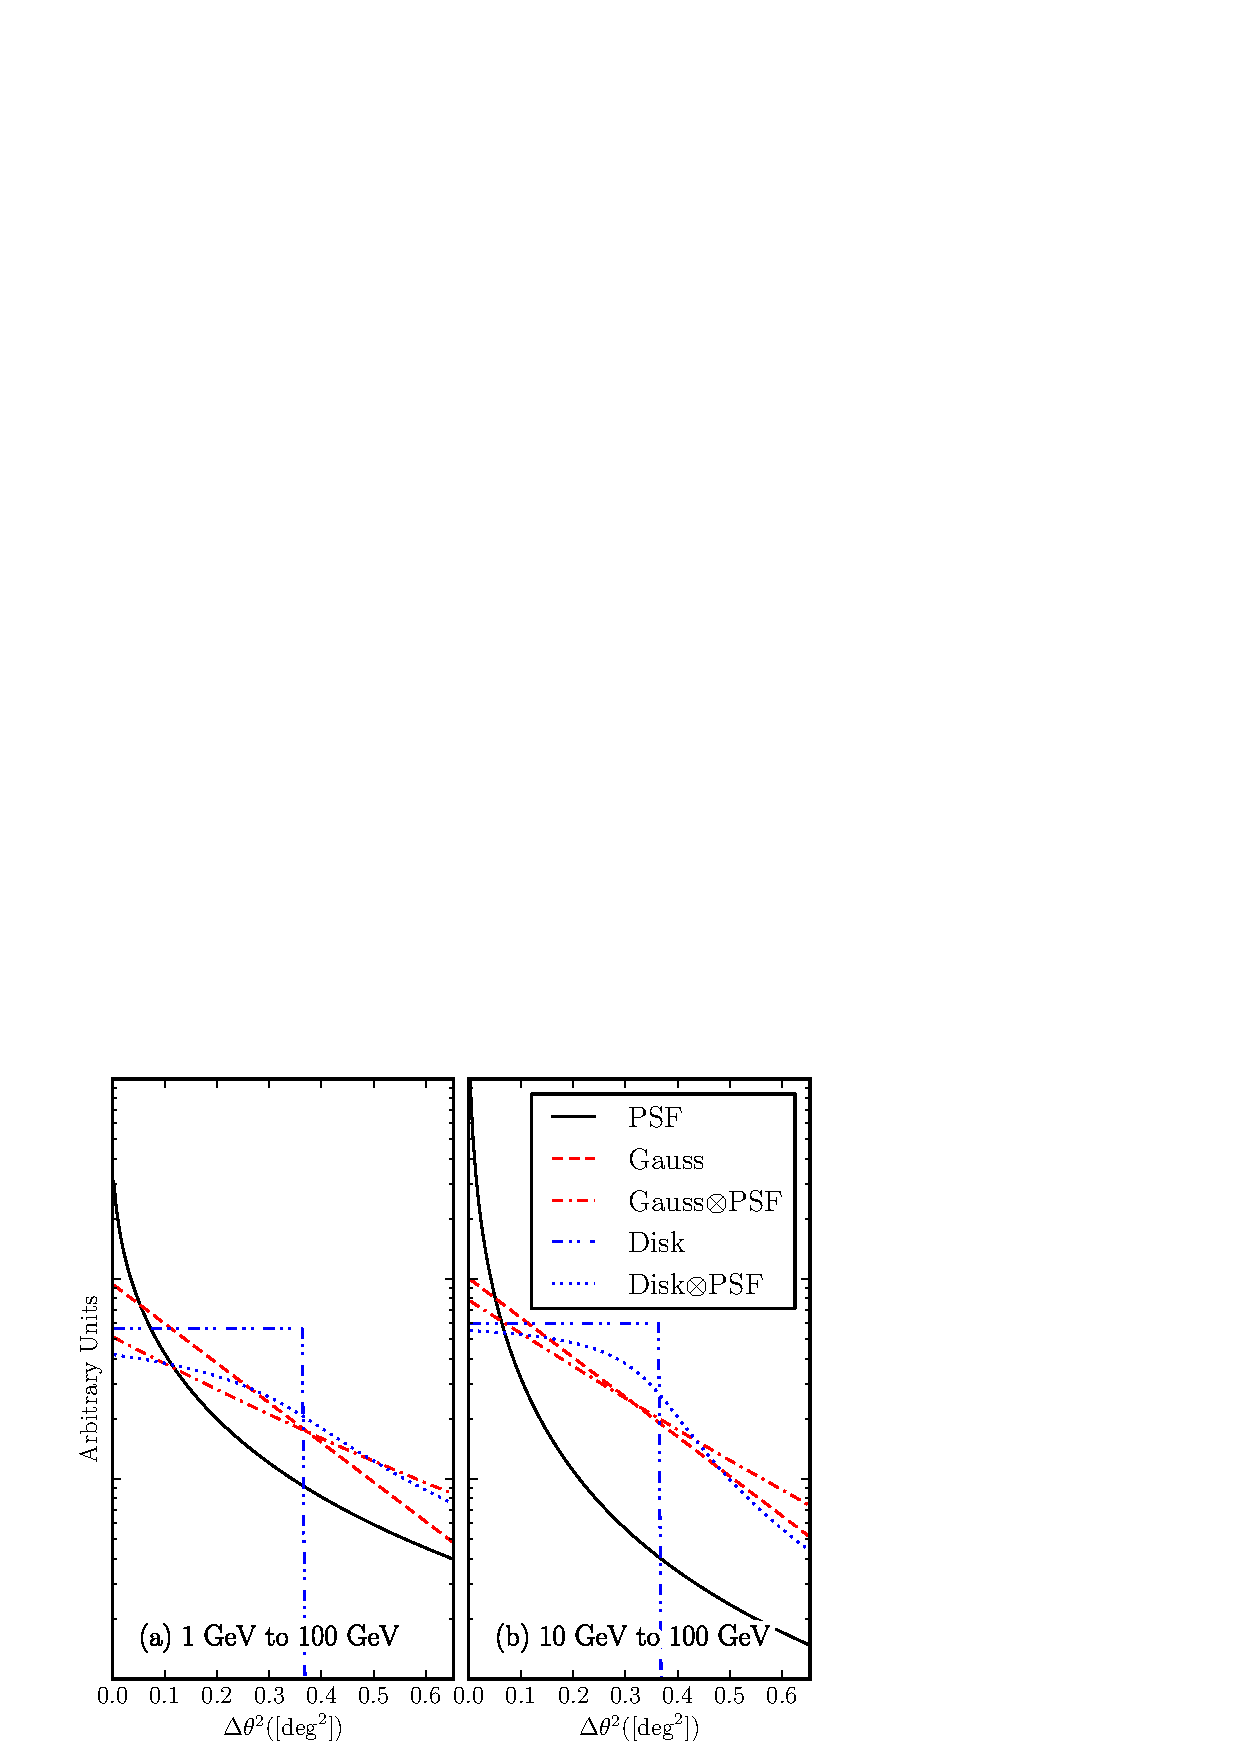
\includegraphics[scale=0.50]{plots/compare_disk_gauss_color.pdf}
    \column{.45\textwidth} 
    \begin{itemize}
      \item Compare Disk, Gauss, and their convolutions with 
      the PSF
      \item For smaller extended sources, little sensitivity
      to spatial shape
    \end{itemize}
  \end{columns}
\end{frame}

\begin{frame}{Table 1: False-Detection Rate}
  \begin{columns}
    \column{.5\textwidth} 
    \includegraphics[scale=0.35]{plots/table_1.pdf}
    \column{.5\textwidth} 
    \begin{itemize}
      \item Simulate point-like sources
      \item Test for extension
      \item Good agreement with Wilk's Theorem
      \item Use $\sqrt{\mathrm{TS}_\mathrm{ext}}$
        as a measure of significance
      \item $\sim 20,000$ Simulations per spectral model!
      \item Test in 1 GeV to 100 GeV + 10 GeV to 100 GeV
        energy range
    \end{itemize}
  \end{columns}
\end{frame}

\begin{frame}{Fig. 3+4: False-Detection Rate (cont)}
  \begin{columns}
    \column{.5\textwidth} 
    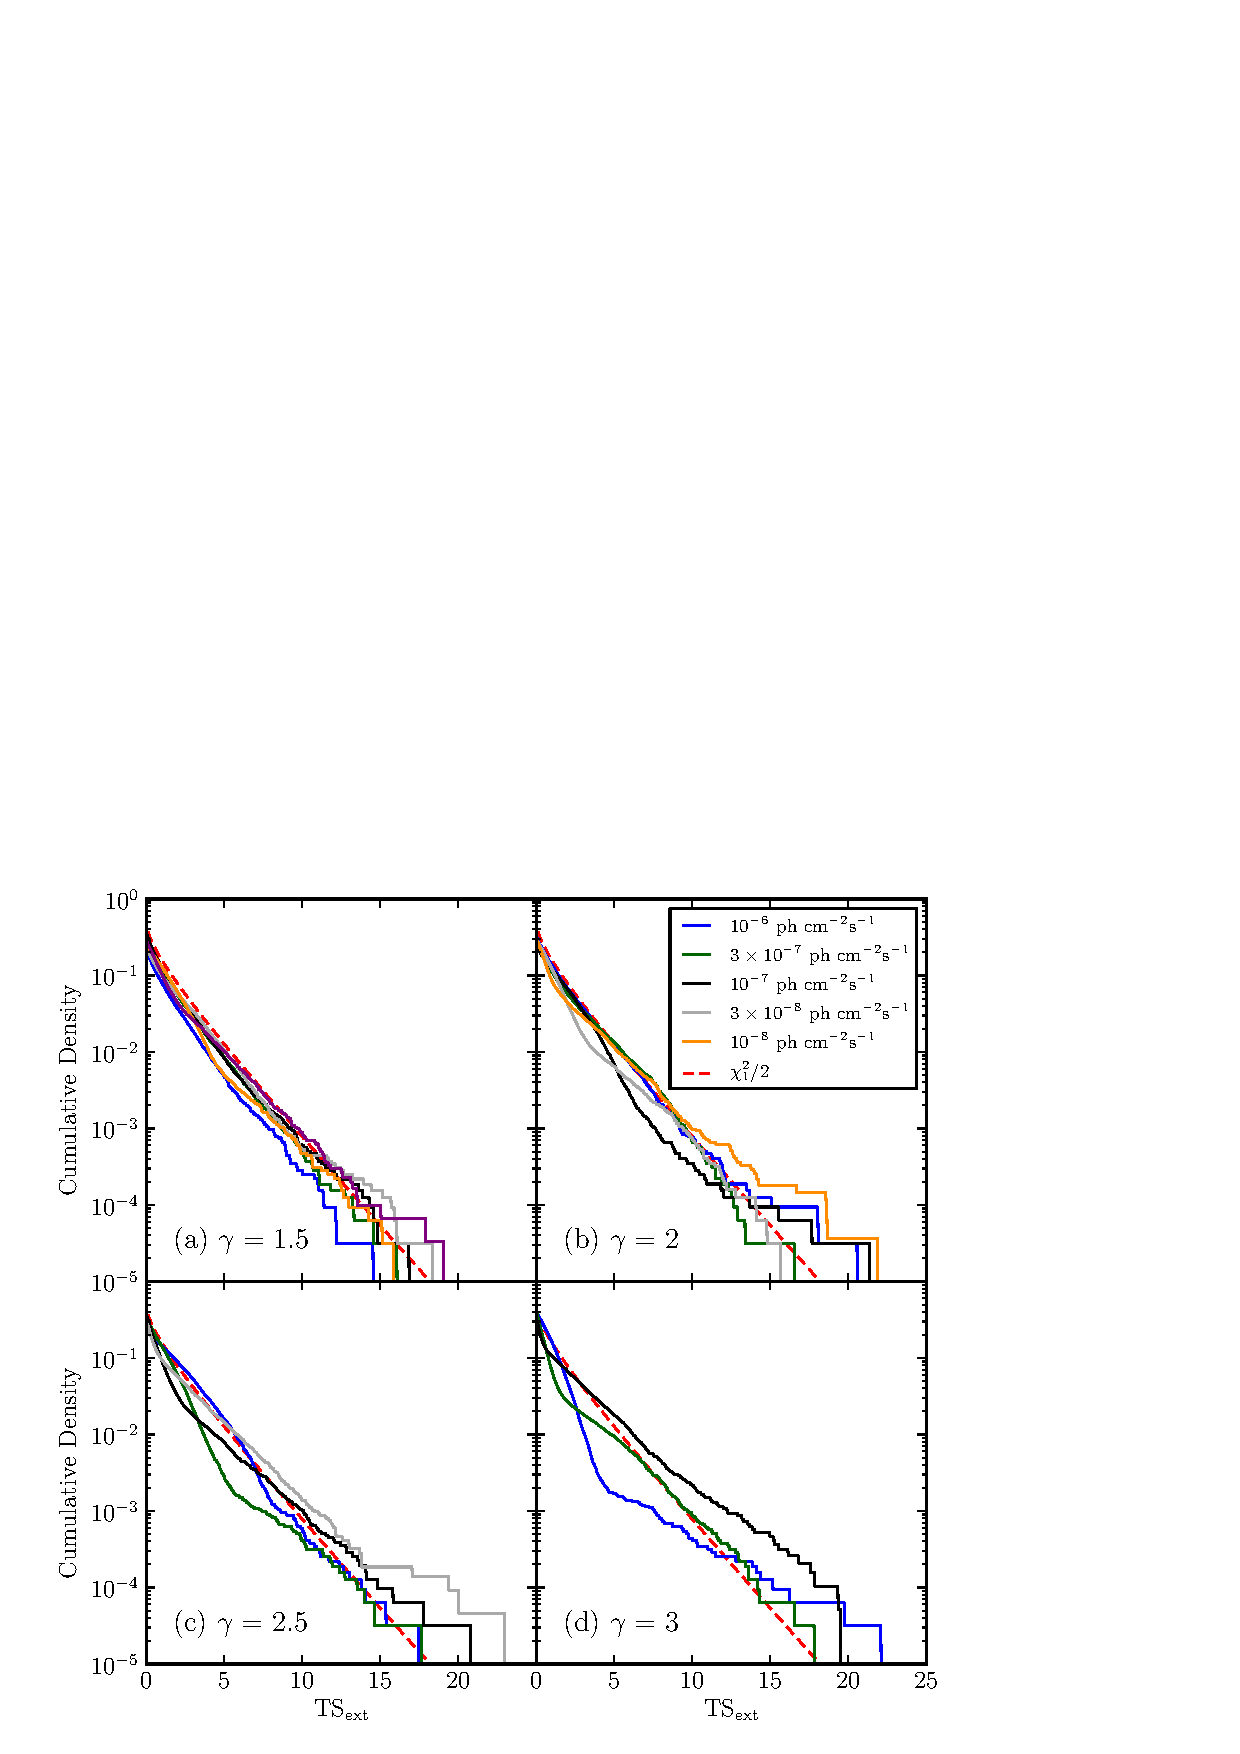
\includegraphics[scale=0.35]{plots/ts_ext_emin_1000_color.pdf}


    Fig 3: 1 GeV to 100 GeV
    \column{.5\textwidth} 
    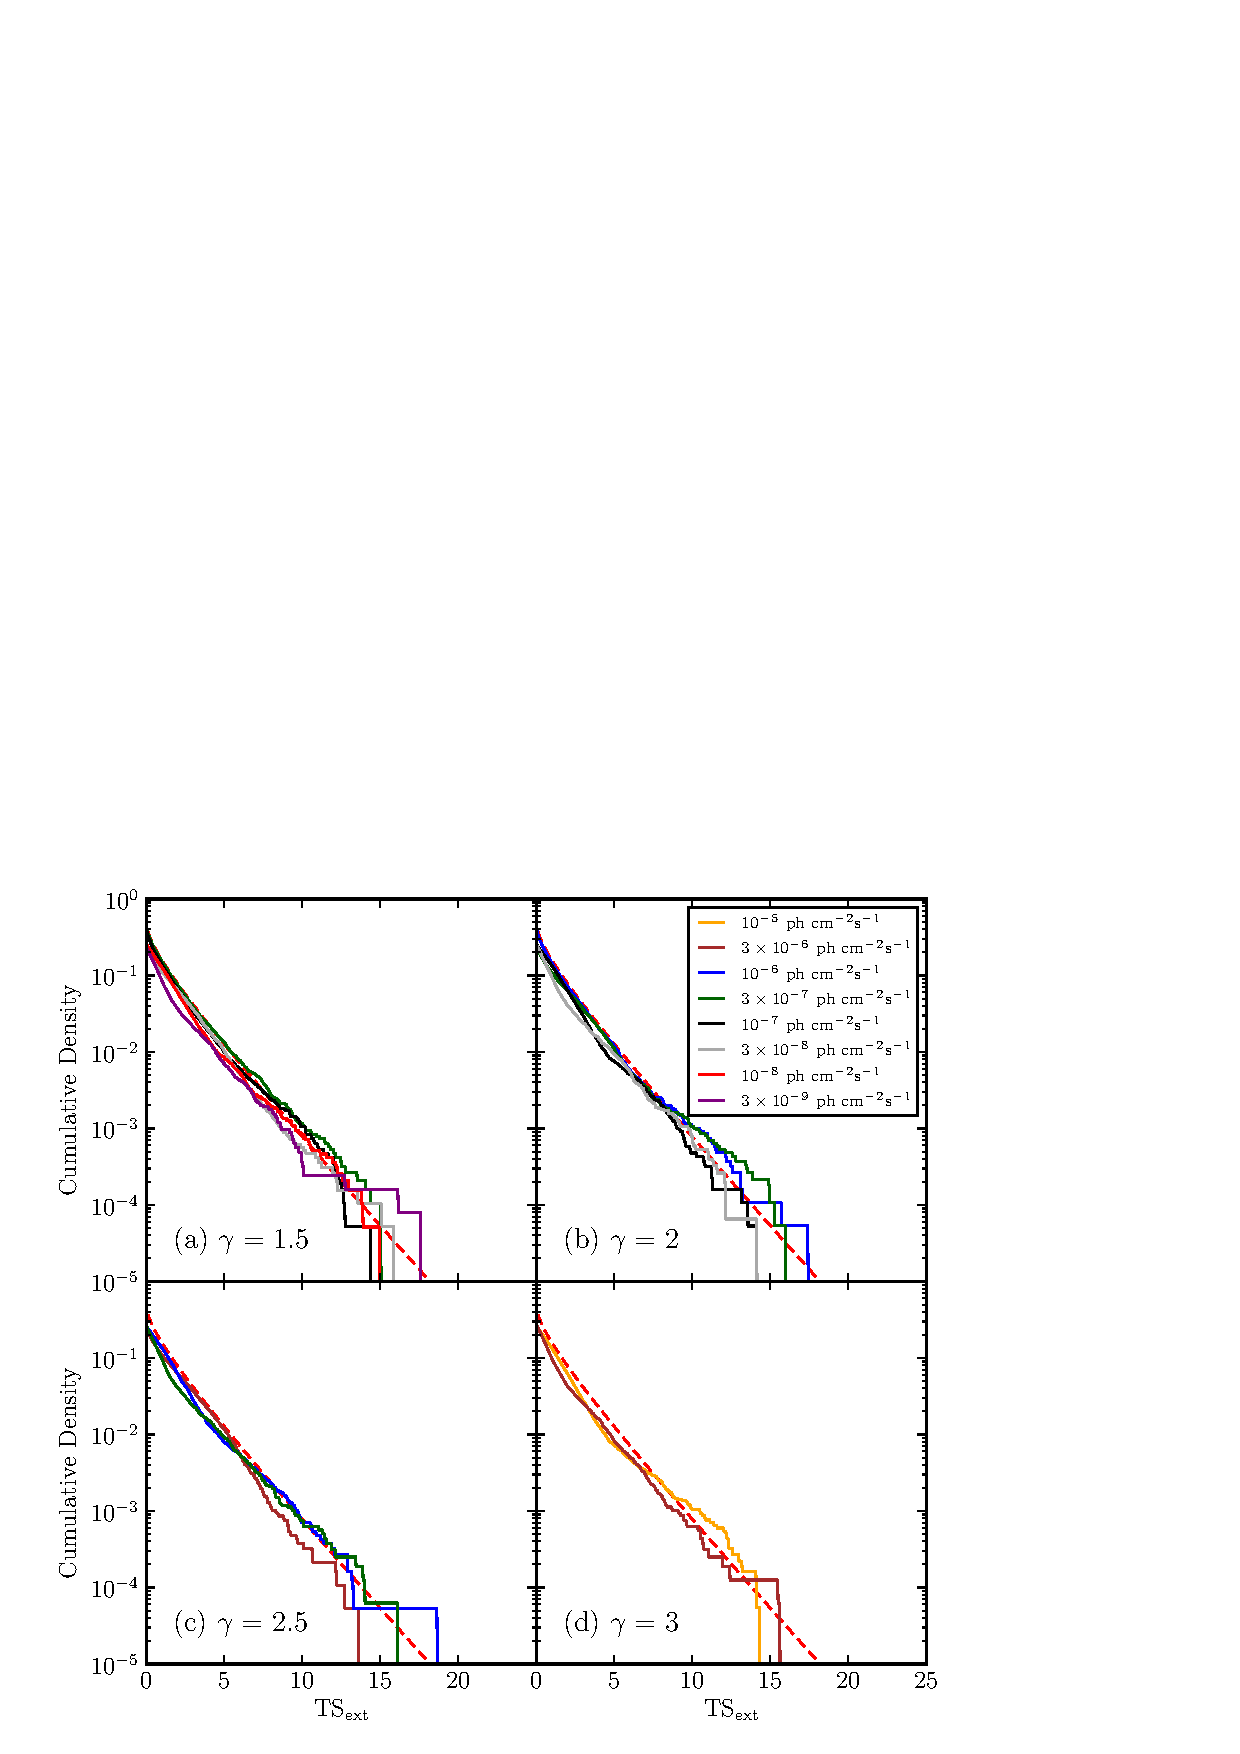
\includegraphics[scale=0.35]{plots/ts_ext_emin_10000_color.pdf}

    Fig 4: 10 GeV to 100 GeV
  \end{columns}
\end{frame}

\begin{frame}{Fig. 5: Detection Threshold}
  \begin{columns}
    \column{.6\textwidth}
    \includegraphics[scale=0.5]{plots/index_sensitivity_color.pdf}
    \column{.4\textwidth}
    \begin{itemize}
      \item Detetion threshold to extension
      \item $\langle\text{TS}_\text{ext}\rangle=16$
      \item Vary spectra, background, energy range
      \item More sensitive to Harder sources
      \item Not sensitive to very small extended sources
    \end{itemize}
  \end{columns}
\end{frame}

\begin{frame}{Fig. 6: Detection Threshold (cont)}
  \begin{columns}
    \column{.60\textwidth}
    \includegraphics[scale=0.45]{plots/all_sensitivity_color.pdf}
    \column{.40\textwidth}
    \begin{itemize}
      \item Compute sensitivty for 
    \begin{itemize}
      \item different background levels
      \item energy ranges.
      \item Spectral Indices
    \end{itemize}
    \item Little index dependence to sensitivity 
      for hard or larger sources
      \item Overlay extended sources 
      $\rightarrow$ Good we are sensitive to them
    \end{itemize}
  \end{columns}
\end{frame}

\begin{frame}{Table 2: Detection Threshold (cont)}
  \includegraphics[scale=0.5]{plots/threshold_table.pdf}
\end{frame}

\begin{frame}{Fig. 7: Detection Threshold (cont)}
  \begin{columns}
    \column{.6\textwidth}
    \includegraphics[scale=0.50]{plots/time_sensitivity_color.pdf}
    \column{.4\textwidth}
    \begin{itemize}
      \item Compute sensitivty after 10 years.
      \item Improvement better than $\sqrt{n}$ for
      small sources
      \item True becasue sensitivity dominated by
      high energy $\rightarrow$ not background limited
    \end{itemize}
  \end{columns}
\end{frame}

\begin{frame}{Fig. 8: Effects of Source Confusion}

Is it an extended source or two point sources?

        \begin{equation*}
          \text{TS}_\text{2pts} =  
          2 \log(\mathcal{L}_\text{2pts}/\mathcal{L}_\text{ps})
        \end{equation*}

  \begin{columns}
    \column{.60\textwidth}
    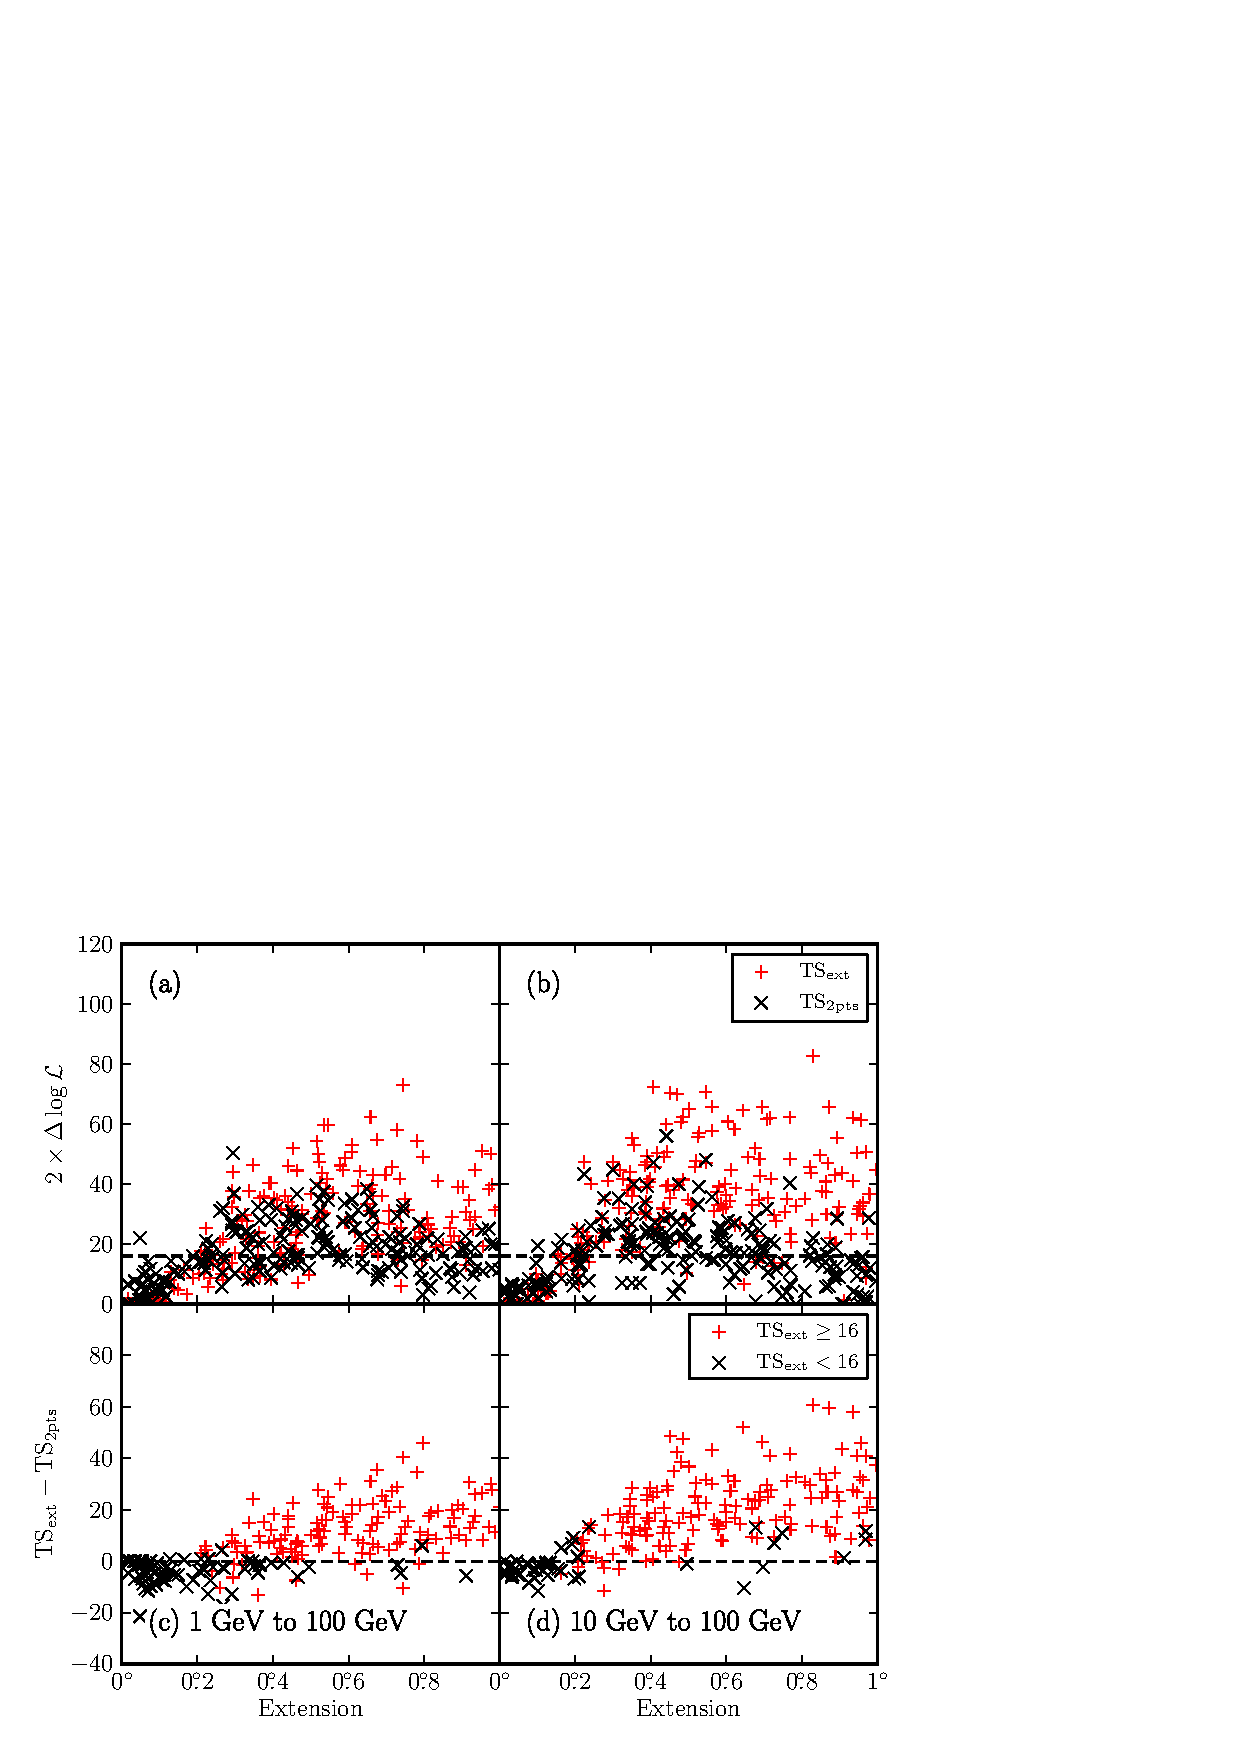
\includegraphics[scale=0.40]{plots/confusion_extended_plot_color.pdf}
    \column{.40\textwidth}
    \begin{enumerate}
      \item Non-nested model comparison
      \item Simulate extended sources. 
      \item Fit as point-like sources.
      \item Can easily fit an extended
      source as two point-like sources
    \end{enumerate}
  \end{columns}
\end{frame}


\begin{frame}{Fig. 9: Effects of Source Confusion (cont)}

  \begin{columns}

    \column{.65\textwidth}
    \includegraphics[scale=0.45]{plots/confusion_2pts_plot_color.pdf}
    \column{.35\textwidth}
    \begin{enumerate}
      \item Simulate point-like sources. 
      \item Fit for extension.
      \item Not likely to confuse two point-like sources
      as an extended source
    \end{enumerate}
  \end{columns}
\end{frame}


\begin{frame}{Fig. 10: $\text{TS}_\text{ext}$ for 2LAC AGN}
  \begin{columns}
    \column{.6\textwidth}
    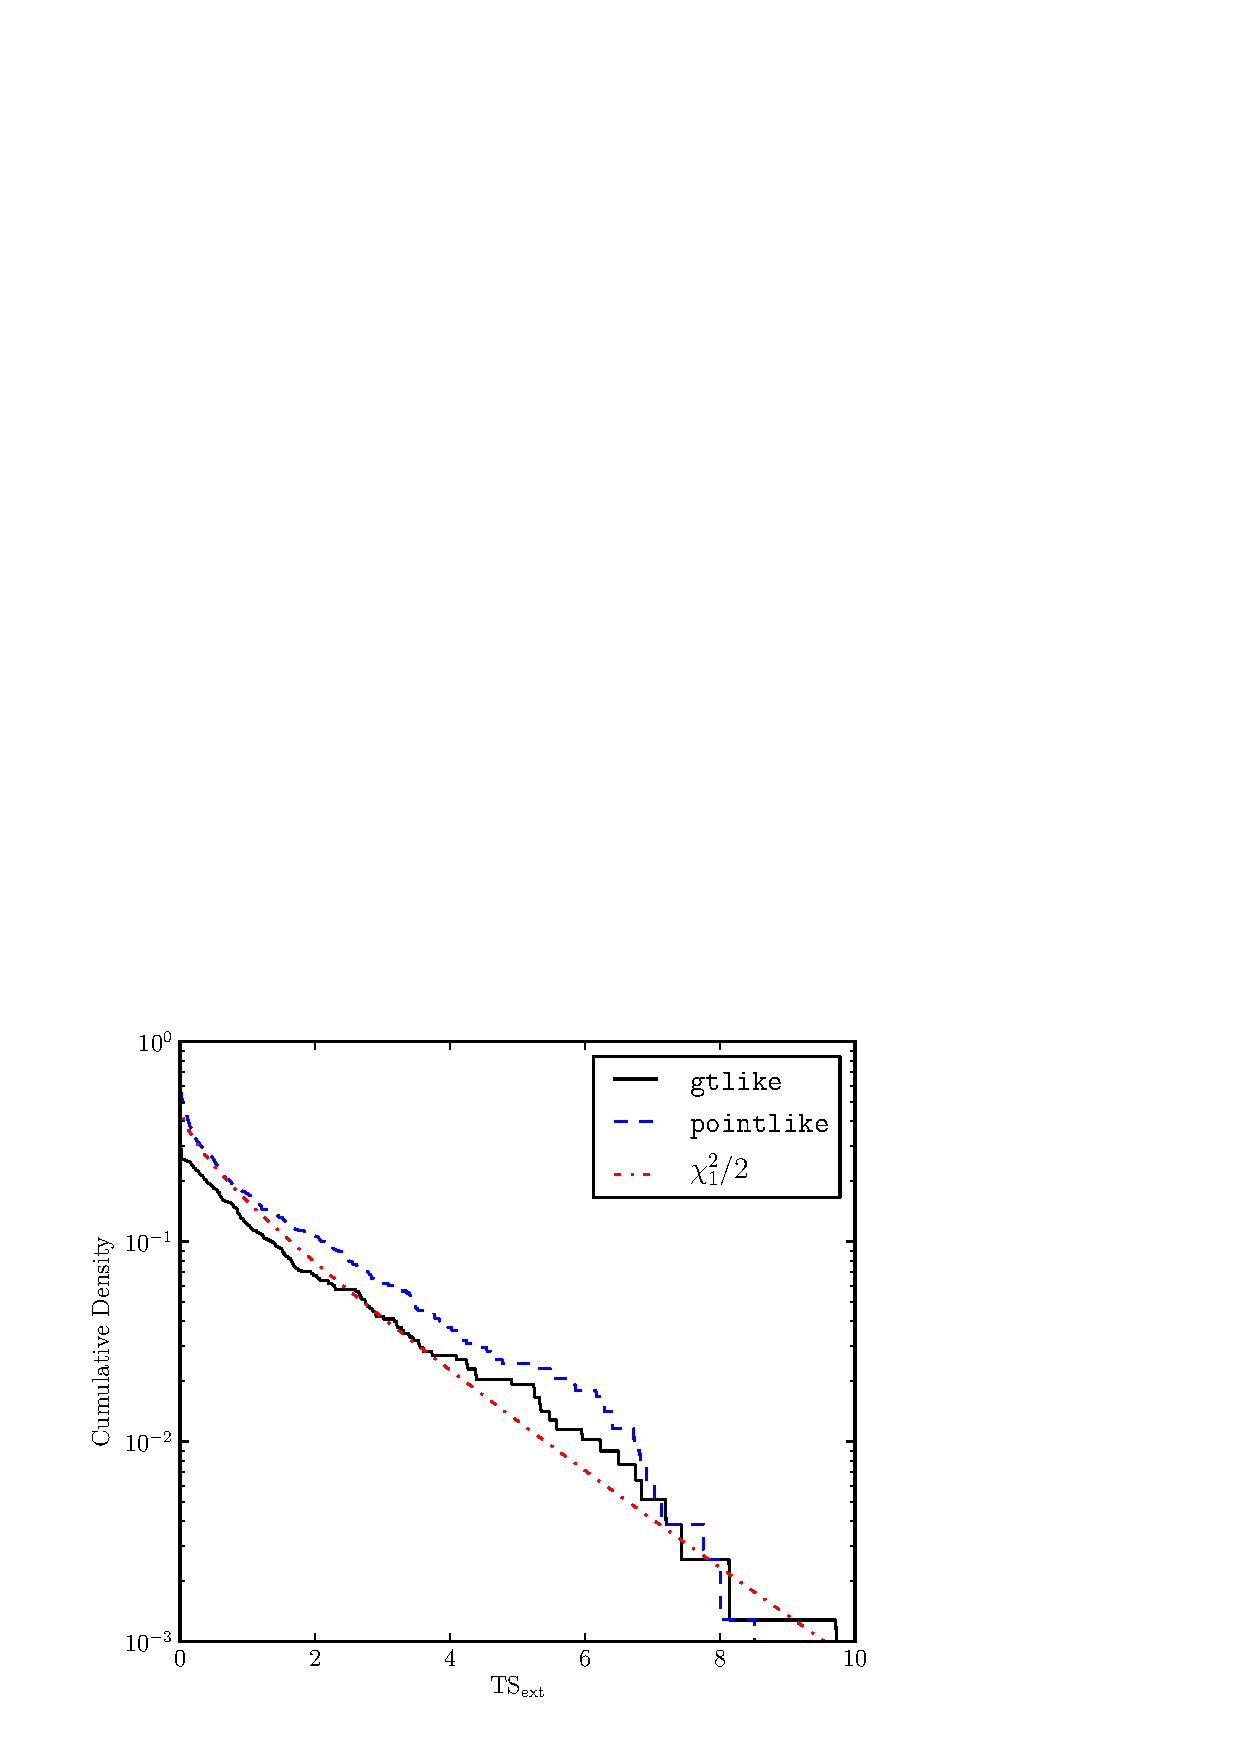
\includegraphics[scale=0.45]{plots/agn_color.pdf}
    \column{.4\textwidth}
    \begin{itemize}
      \item Use point-like AGN to validate extended source analysis
      \item Test clean 2LAC AGN for extension
      \item Don't find AGN to be extended!
    \end{itemize}
  \end{columns}
\end{frame}

\begin{frame}{Fig. 1 + 11: IC~443}
\begin{itemize}
\item IC443 is the Most significantly extended source
\item Below are diagnostic plots
\end{itemize}
  \begin{columns}
    \column{.5\textwidth}
      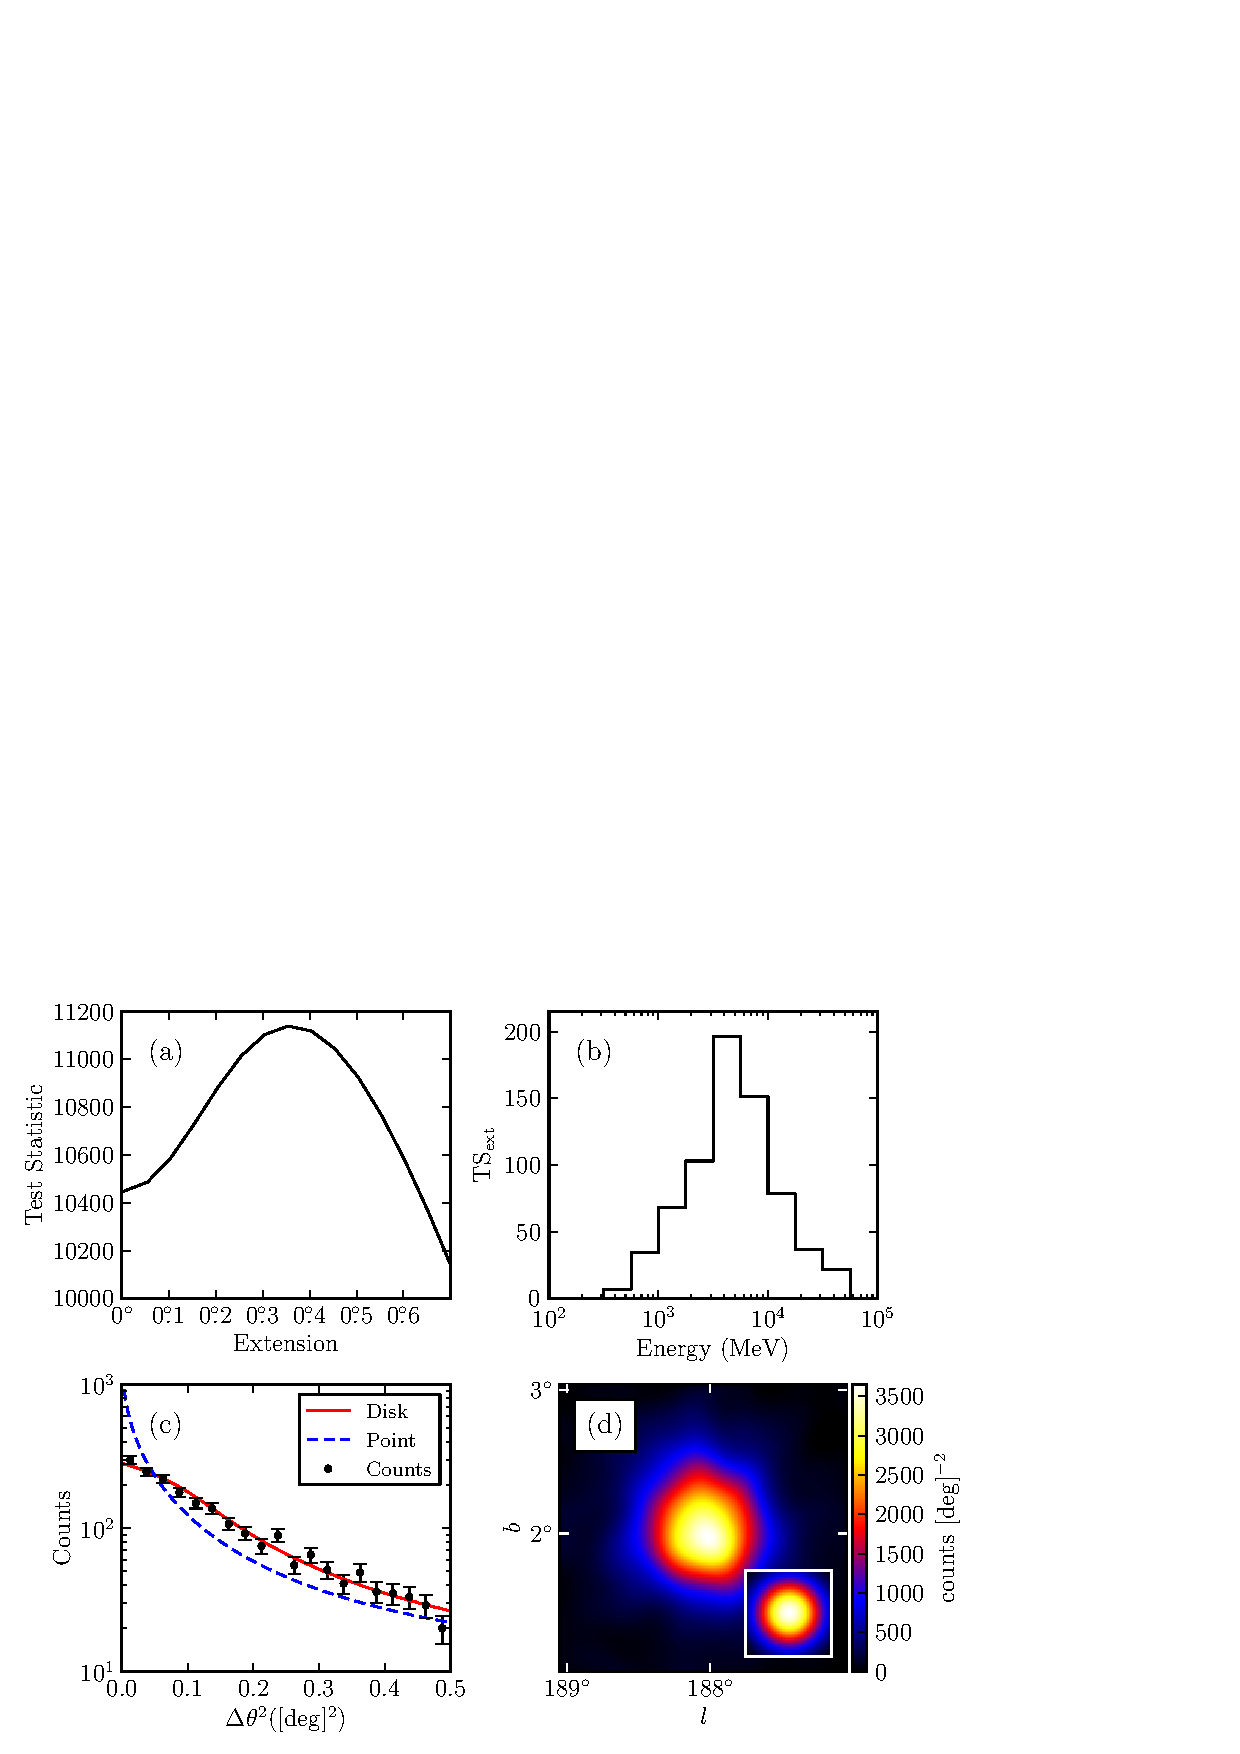
\includegraphics[scale=0.35]{plots/four_plots_ic443_color.pdf}

    \column{.5\textwidth}
      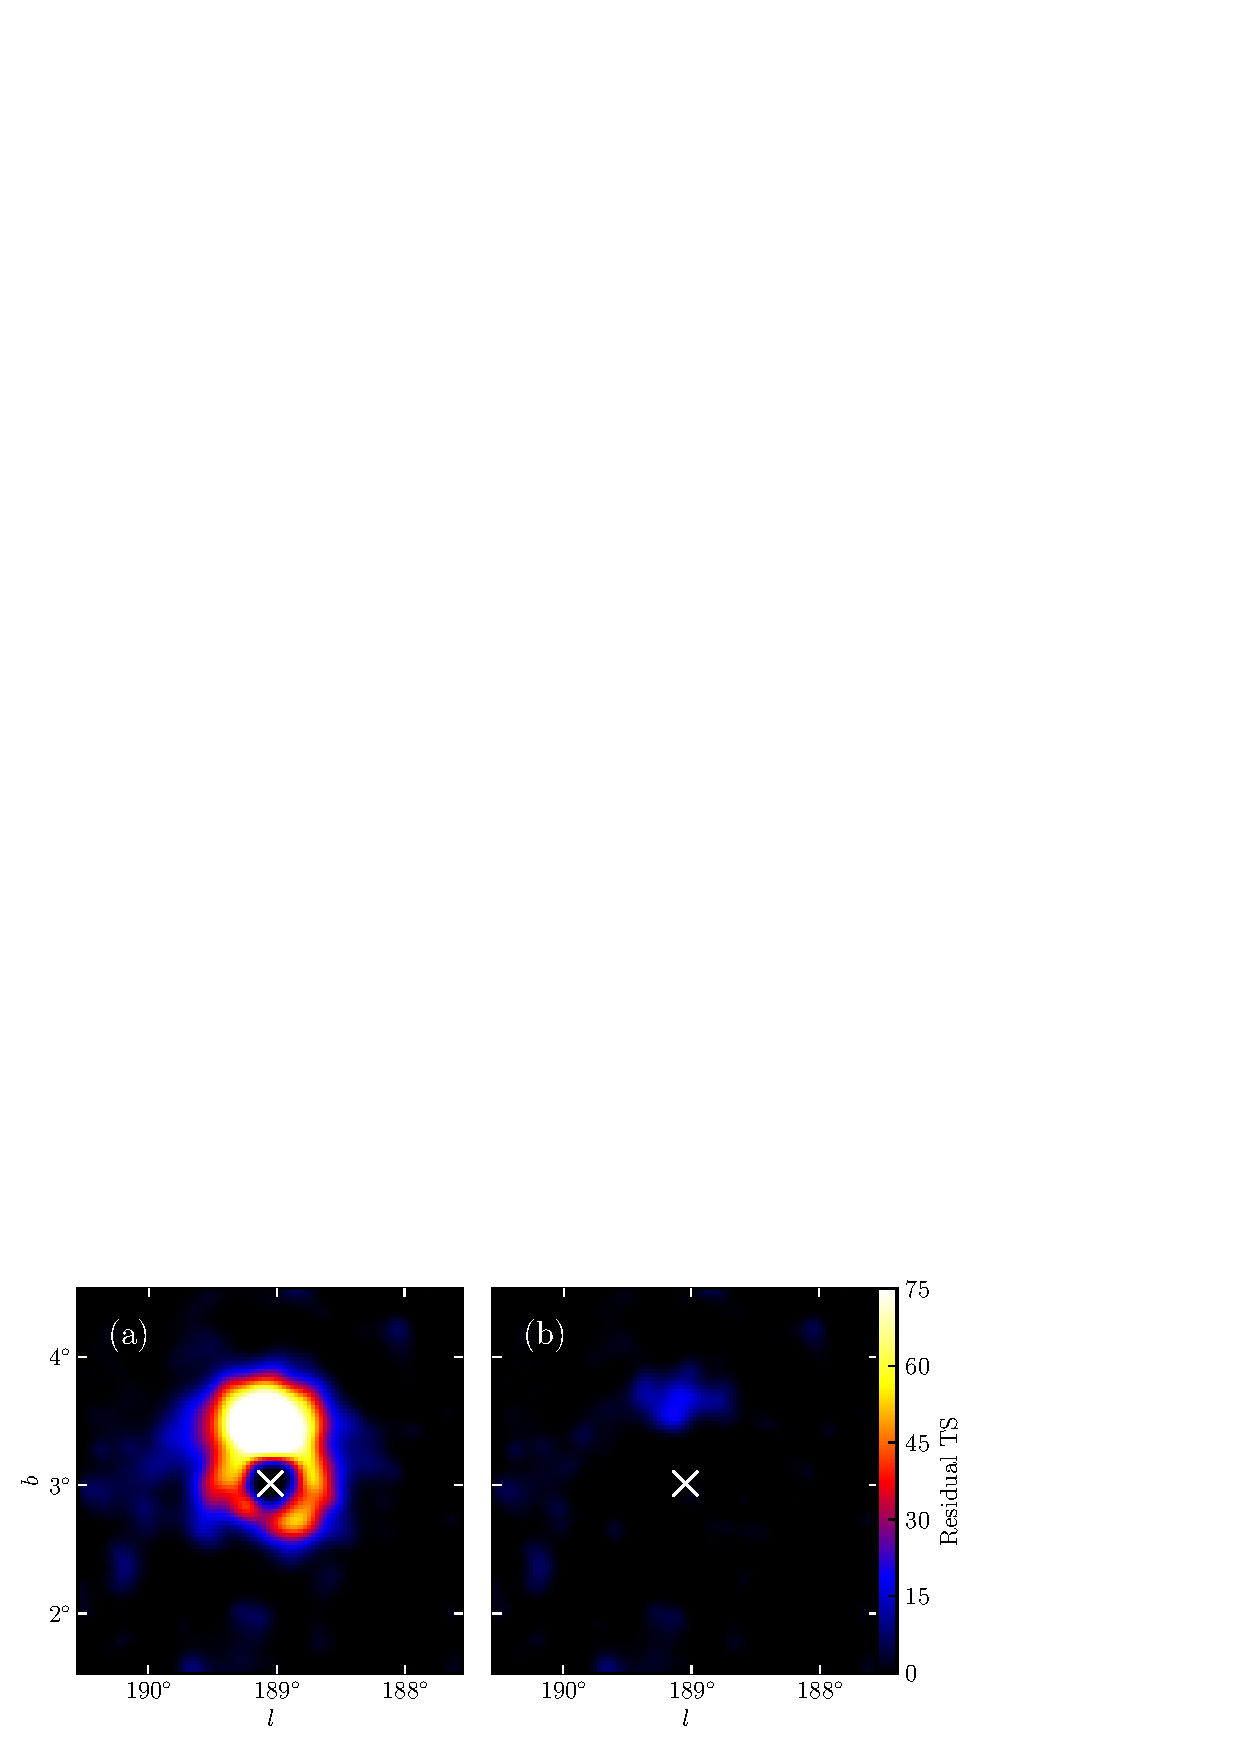
\includegraphics[scale=0.35]{plots/res_tsmap_ic443_color.pdf}

      Residual TS Map 
      \begin{itemize}
      \item (a) IC443 a point source 
      \item (b) IC443 extended
      \end{itemize}
  \end{columns}
\end{frame}



\begin{frame}{Table 3: extended sources in 2FGL}
  \begin{columns}
    \column{.6\textwidth}
    \includegraphics[scale=0.4]{plots/table_reanalysis.pdf}
    \column{.4\textwidth}
    \begin{itemize}
      \item Test 12 extended 2FGL sources for extension
      \item Systematic reanalysis using 2 years of data.
      \item Assume uniform disk
      \item Extended sources are extended!
    \end{itemize}
  \end{columns}
\end{frame}

\begin{frame}{Section 9: Extended Source Search}
  \begin{itemize}
    \item Run a dedicated search 
    \item Try to find previously-unresolved
      extended 2FGL sources
    \item Search for $E>1$ GeV and $E>10$ GeV
    \item Many difficulties in search, discussed at length in text\dots
    \item Publish only good candidates
  \end{itemize}
\end{frame}

\begin{frame}{Fig. 12: Systematics in the plane}
  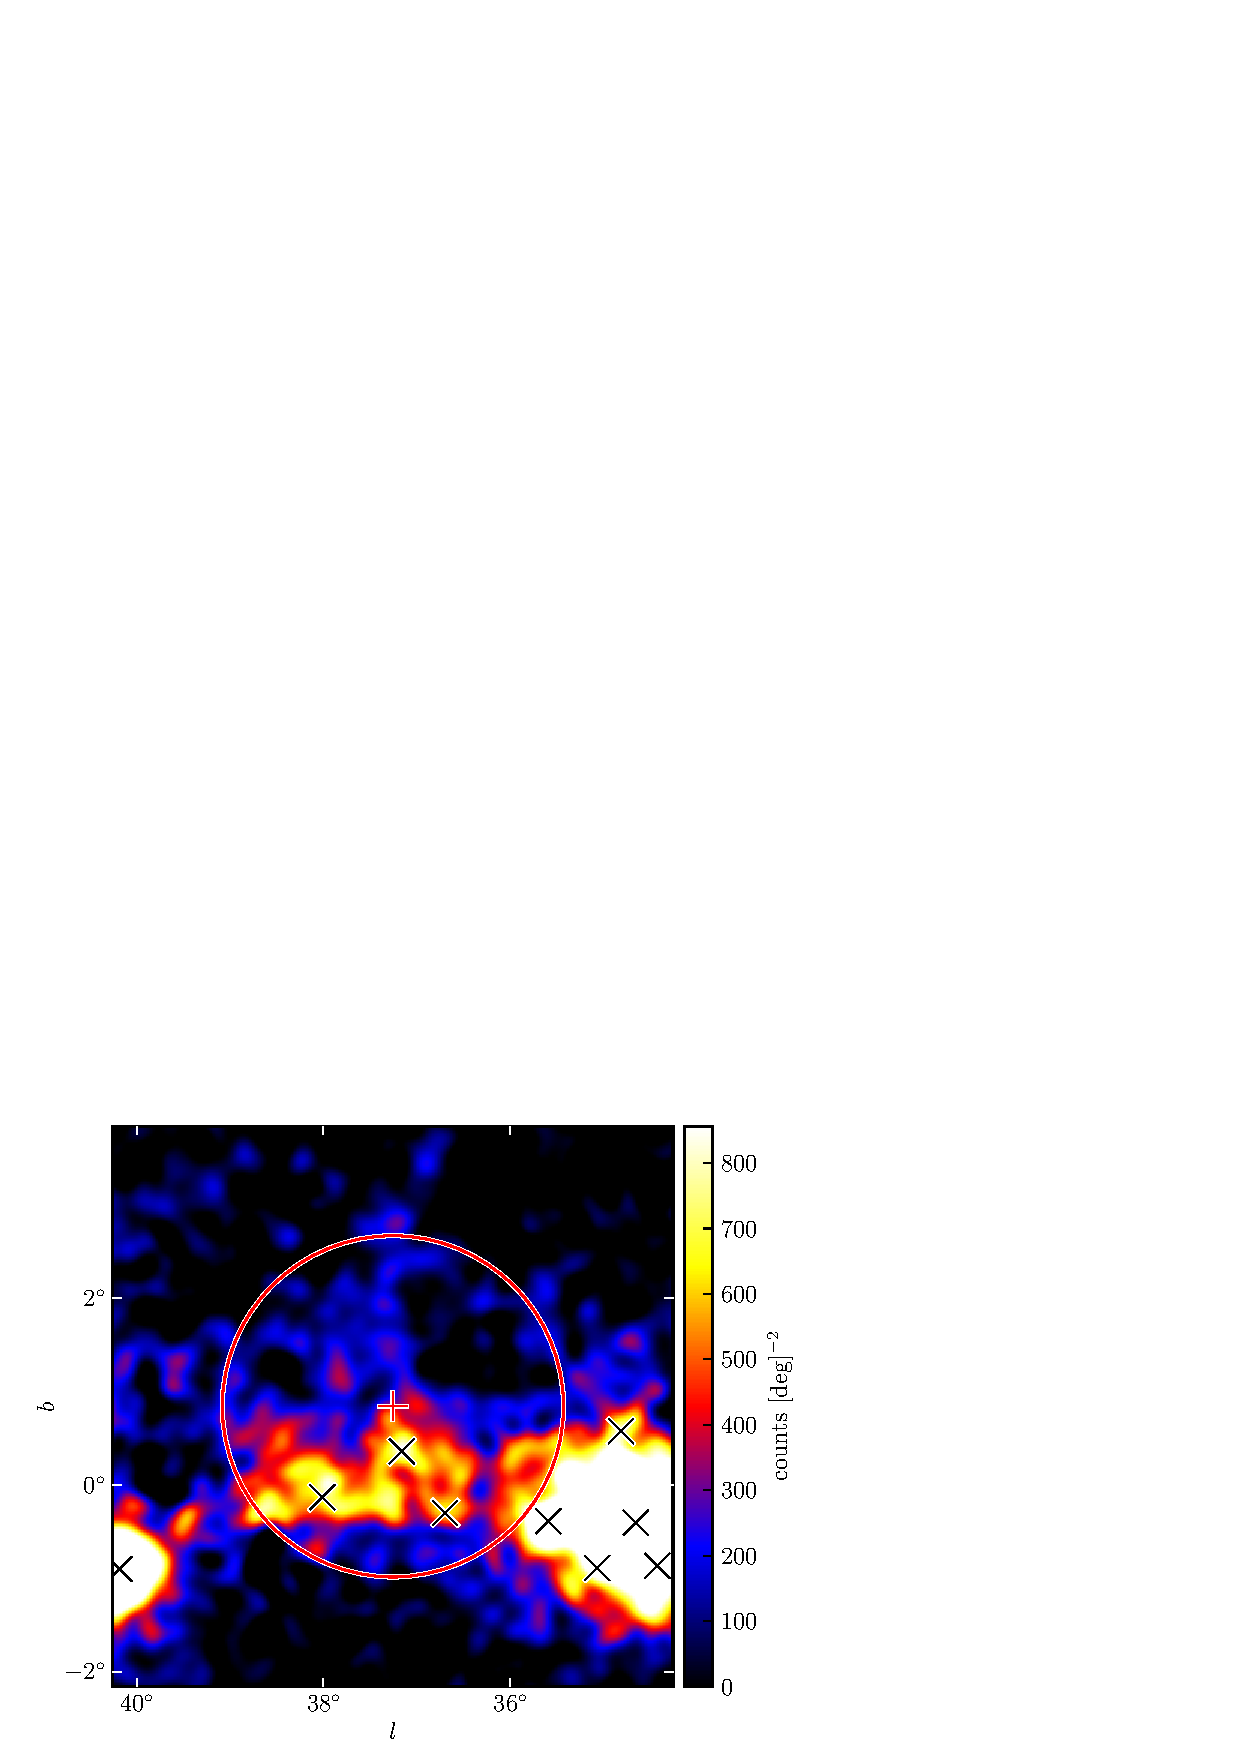
\includegraphics[scale=0.5]{plots/example_bad_fit_color.pdf}
\end{frame}

\begin{frame}{Fig 13: Puppis A}

  \begin{columns}
    \column{.60\textwidth} 
    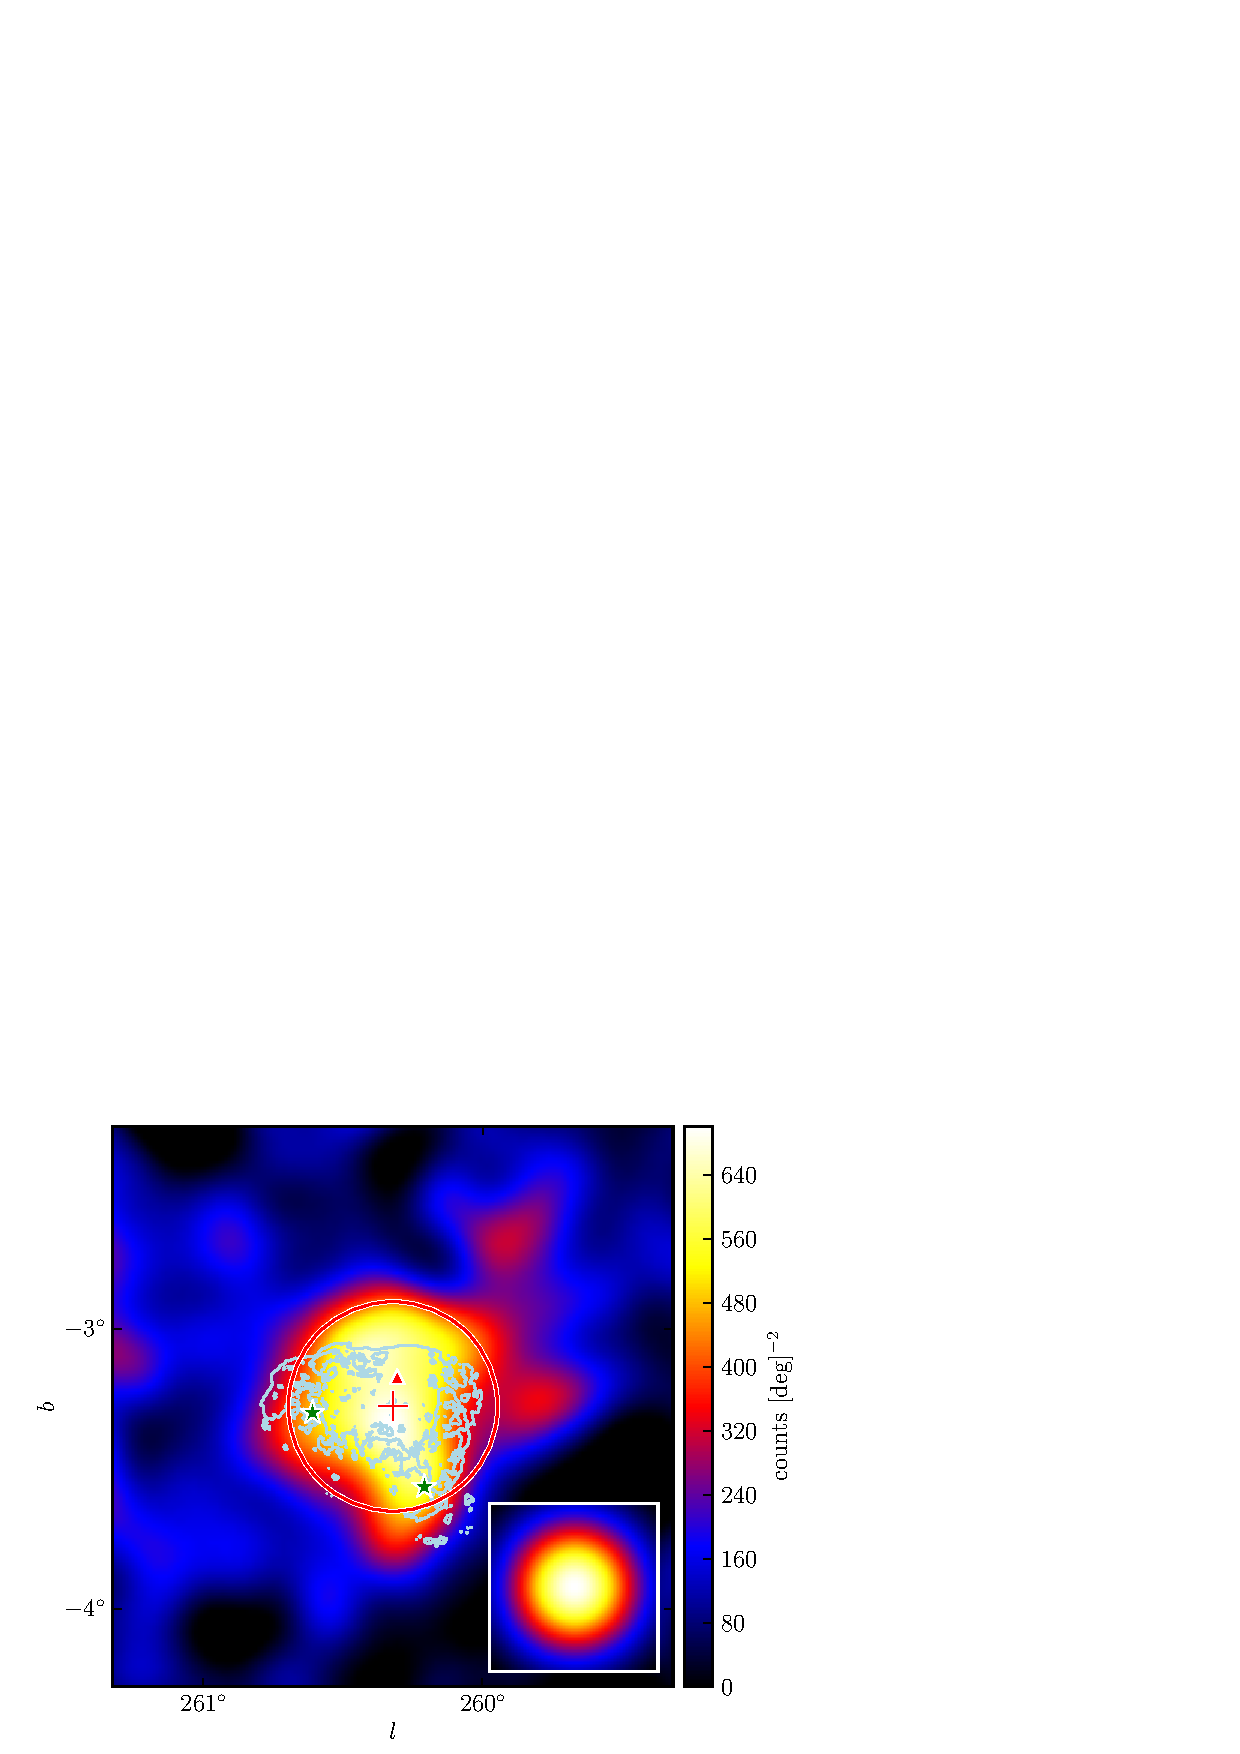
\includegraphics[scale=0.50]{plots/source_Puppis_A_color.pdf}

    \column{.40\textwidth} 
    \begin{itemize}
    \item 1 GeV to 100 GeV
      \item Middle-aged SNR
      \item ROSAT X-ray contours (Petre+1996)
      \item SNR not observed to interact with
      molecular clouds (Paron+2008)
      \item Similar to Cygnus Loop
      \end{itemize}
  \end{columns}
\end{frame}

\begin{frame}{Fig 22: $\gamma$-Cygni}
  \begin{columns}

    \column{.55\textwidth} 
    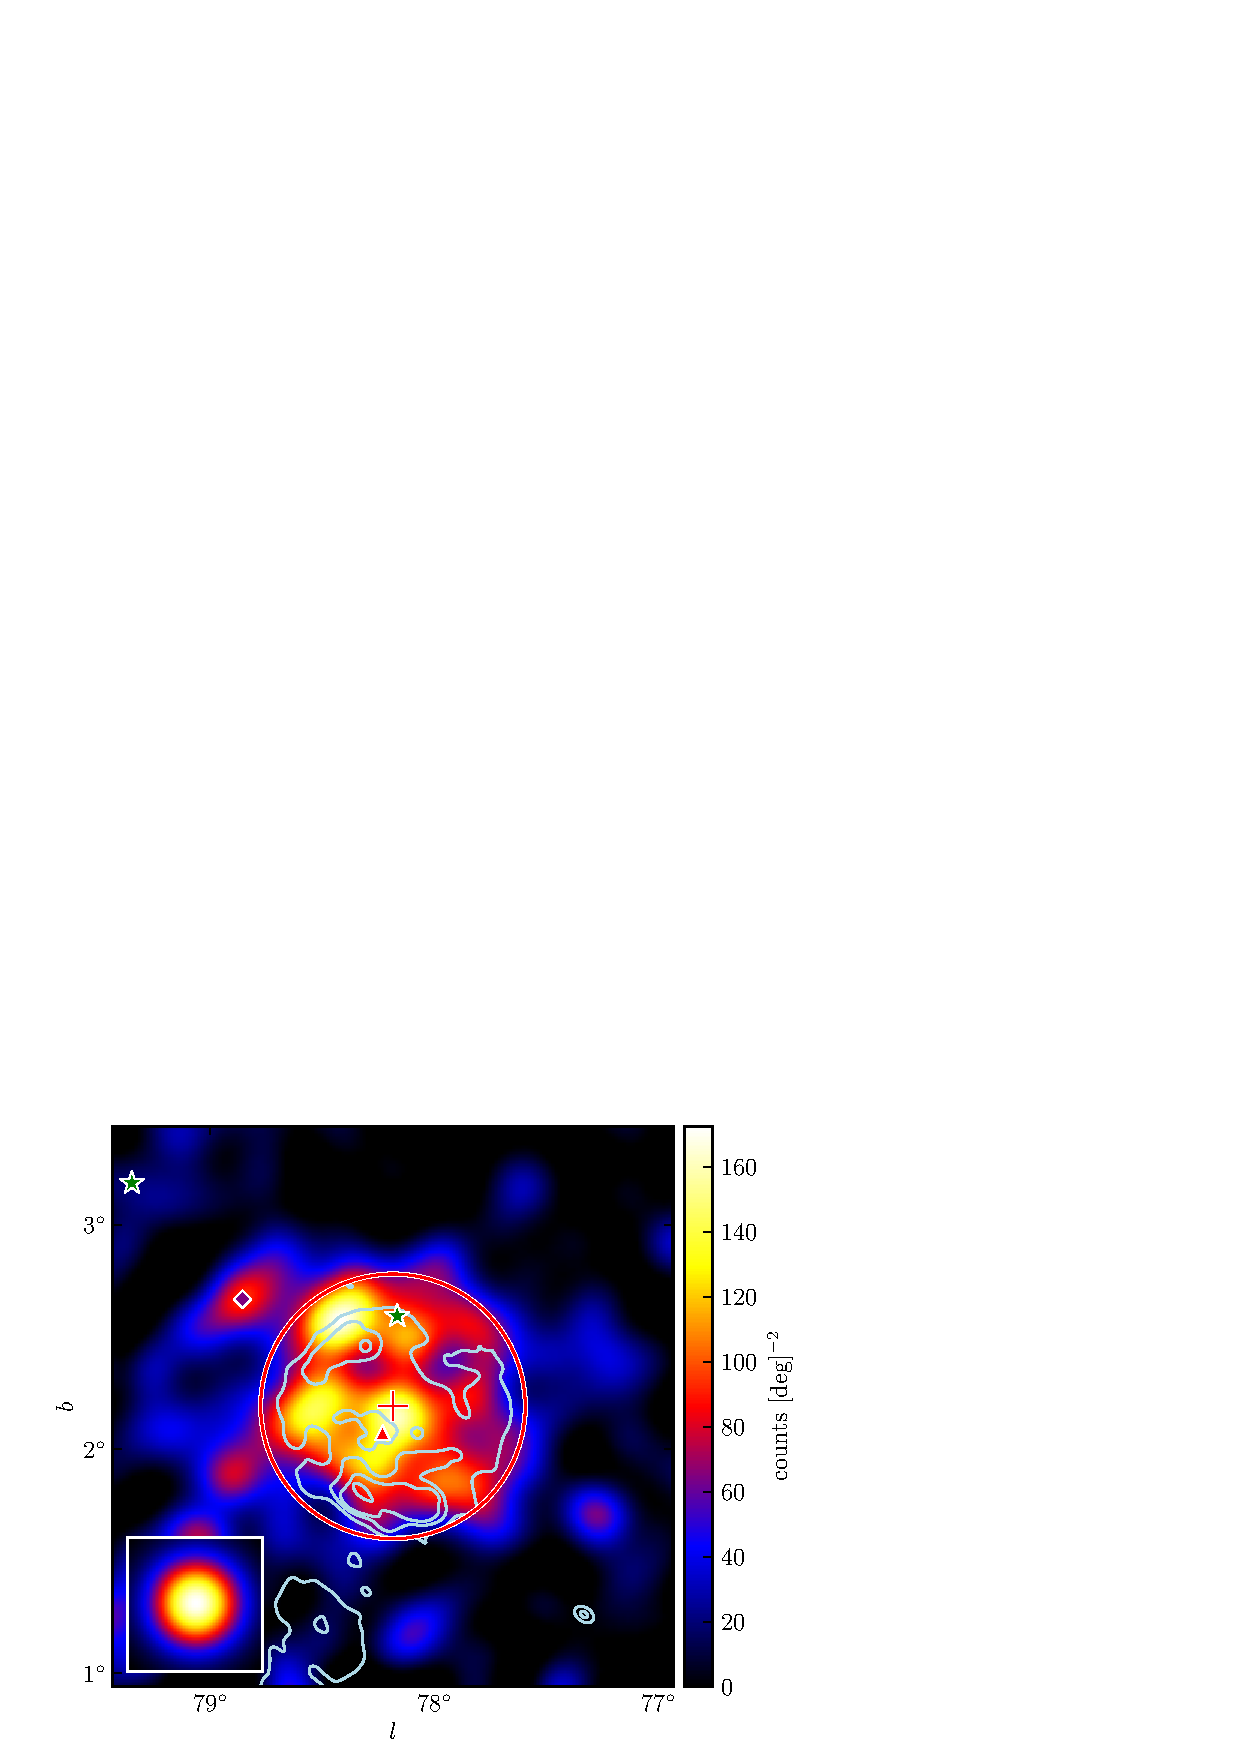
\includegraphics[scale=0.50]{plots/source_Gamma_Cygni_color.pdf}

    \column{.45\textwidth} 

    \begin{itemize}
      \item 10 GeV to 100 GeV
      \item PSR\,J2021+4026 at lower energies
      \item Radio contours (Taylor+2003)
      \item SNR interacting with Molecular cloud
      \item Milagro: $4.2\sigma$ excess at $\sim 30$ TeV (Abdo+2009)
      \item 
        VER\,J2019+407 
        detected by Veritas at 200 GeV (Weinstein 2009)
      \end{itemize}
  \end{columns}
\end{frame}

\begin{frame}{Fig. 14: SED of SNRs}
  \includegraphics[scale=0.65]{plots/snr_seds_color.pdf}
\end{frame}


\begin{frame}{Fig 17. HESS\,J1614$-$518 \& HESS\,J1616$-$508}
  \begin{columns}
    \column{.6\textwidth} 
    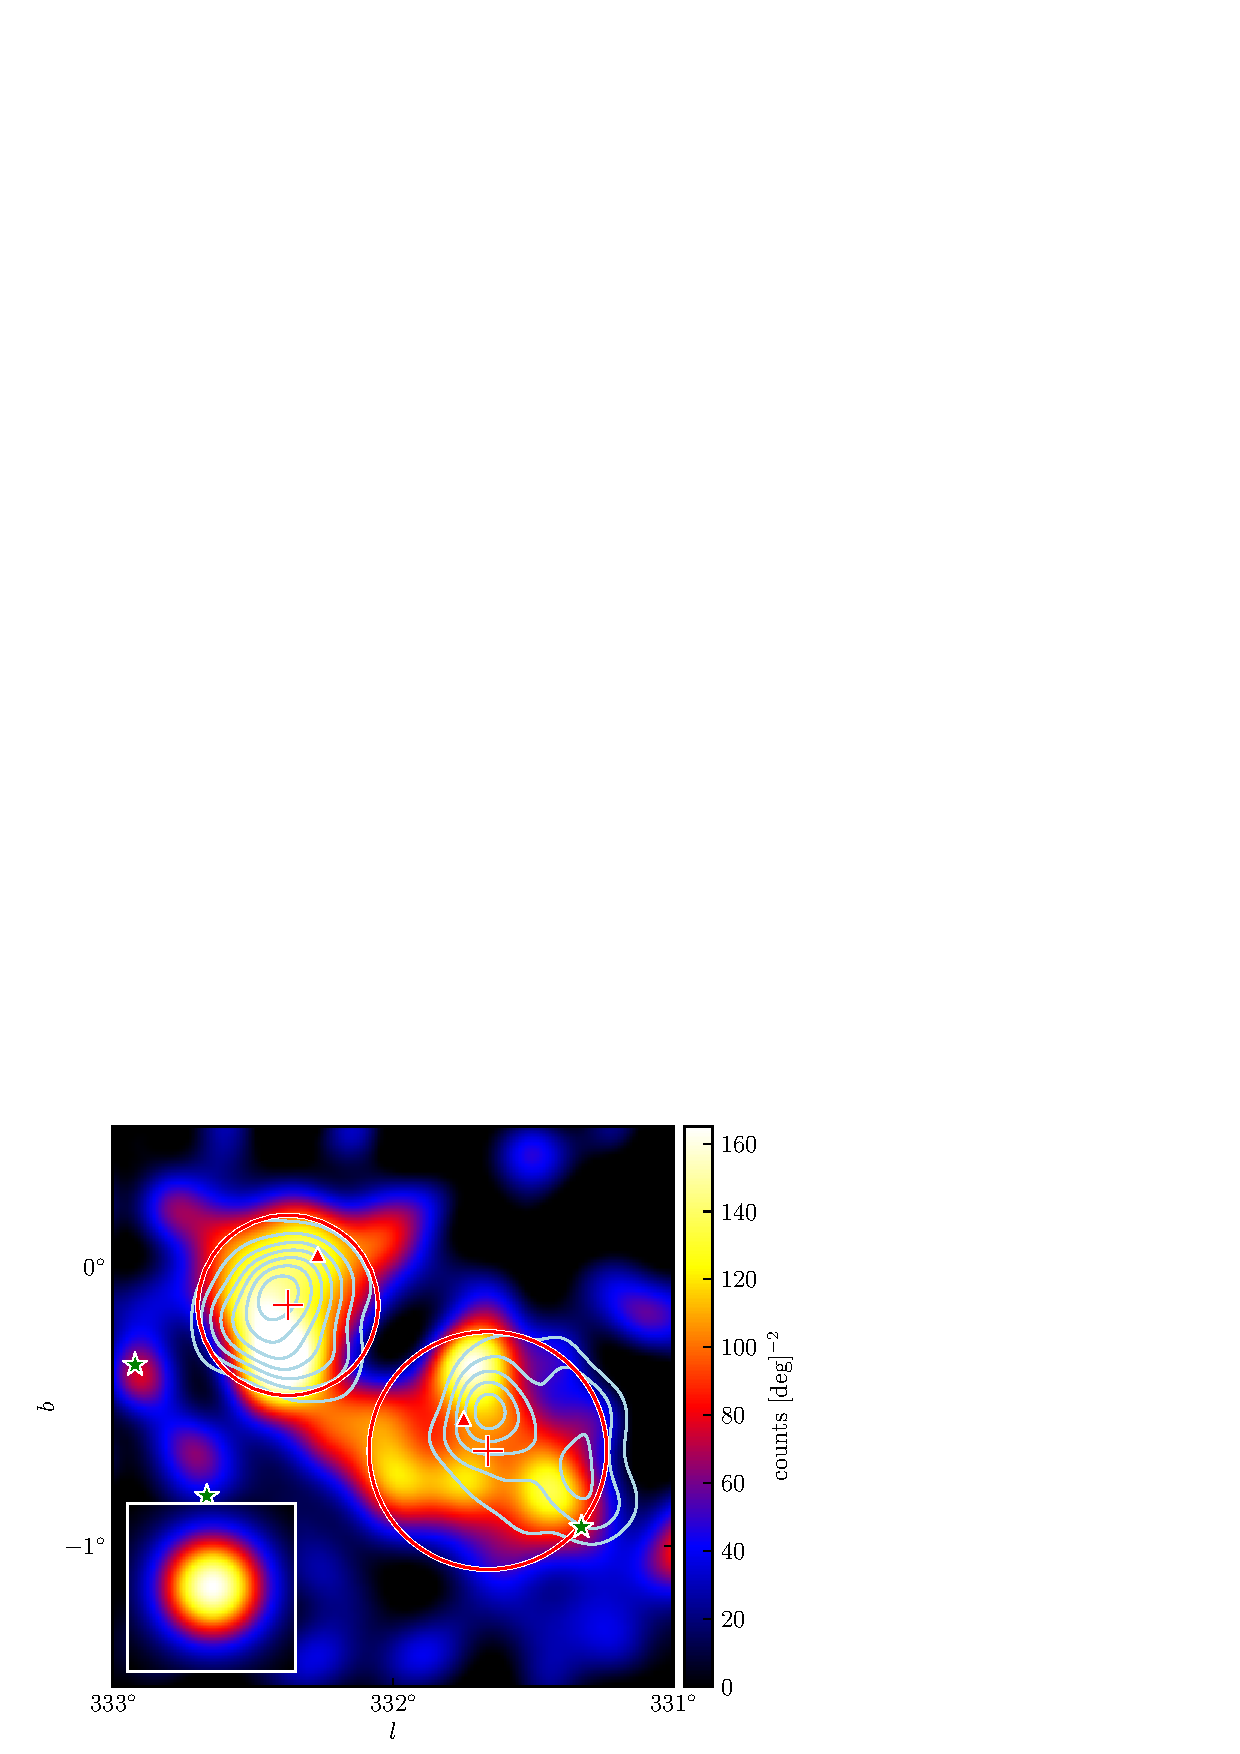
\includegraphics[scale=0.5]{plots/source_HESS_J1614-518_color.pdf}
    \column{.4\textwidth} 
    \begin{itemize}
      \item 10 GeV to 100 GeV
      \item Two nearby LAT extended sources 
      \item both
        coincident with extended TeV sources.
    \end{itemize}
  \end{columns}

  \begin{itemize}
    \item (left): 
      2FGL\,J1615.0$-$5051 $\rightarrow$ HESS\,J1616$-$508
    \item (right):
      2FGL\,J1615.2$-$5138 $\rightarrow$ HESS\,J1614$-$518
  \end{itemize}

\end{frame}

\begin{frame}{2FGL\,J1615.0$-$5051 $\rightarrow$ HESS\,J1616$-$508}
  \begin{columns}
    \column{.4\textwidth} 
    % from http://www.mpi-hd.mpg.de/hfm/HESS/pages/home/som/2007/01/
  \includegraphics[scale=0.45]{plots/Som_1_07_p1.jpg}
    \column{.7\textwidth} 
  \begin{itemize}
    \item 2 nearby SNRs: RCW103 and Kes~32 - not spatially coincident (Aharonian+2006) 
    \item 3 Nearby Pulsars: only 
      PSR\,J1617$-$5055 energetically powerful enough
      \begin{itemize}
        \item 9' away $\rightarrow$ offset PWN?
        \item {\em Chandra} detected $\sim 1'$ PWN 
        \item not oriented towards HESS\,J1616$-$508
        \end{itemize}
      \item Other diffuse emission in region (Kargaltsev+2009)
    \end{itemize}
  \end{columns}
\end{frame}

\begin{frame}{2FGL\,J1615.2$-$5138 $\rightarrow$ HESS\,J1614$-$518}

  \begin{columns}
    \column{.4\textwidth} 
    \includegraphics[scale=0.3]{plots/Som_9_08_p1.jpg}
    \column{.7\textwidth} 
    \begin{itemize}
      \item 5 nearby pulsars, but none powerful enough (Rowell+2008)
      \item Open cluster Pisim 22 
      \item Suzaku: 2 X-ray sources, one towards peak 
        of HESS\,J1614$-$518 and one coincident with Pisim 22
        (Matsumoto+2008)
      \item SNR? PWN? Acceleration in Stellar Winds of Pisim 22?
    \end{itemize}
  \end{columns}
\end{frame}

\begin{frame}{Fig. 19: HESS\,J1632-478}
  \begin{columns}
    \column{.65\textwidth} 
    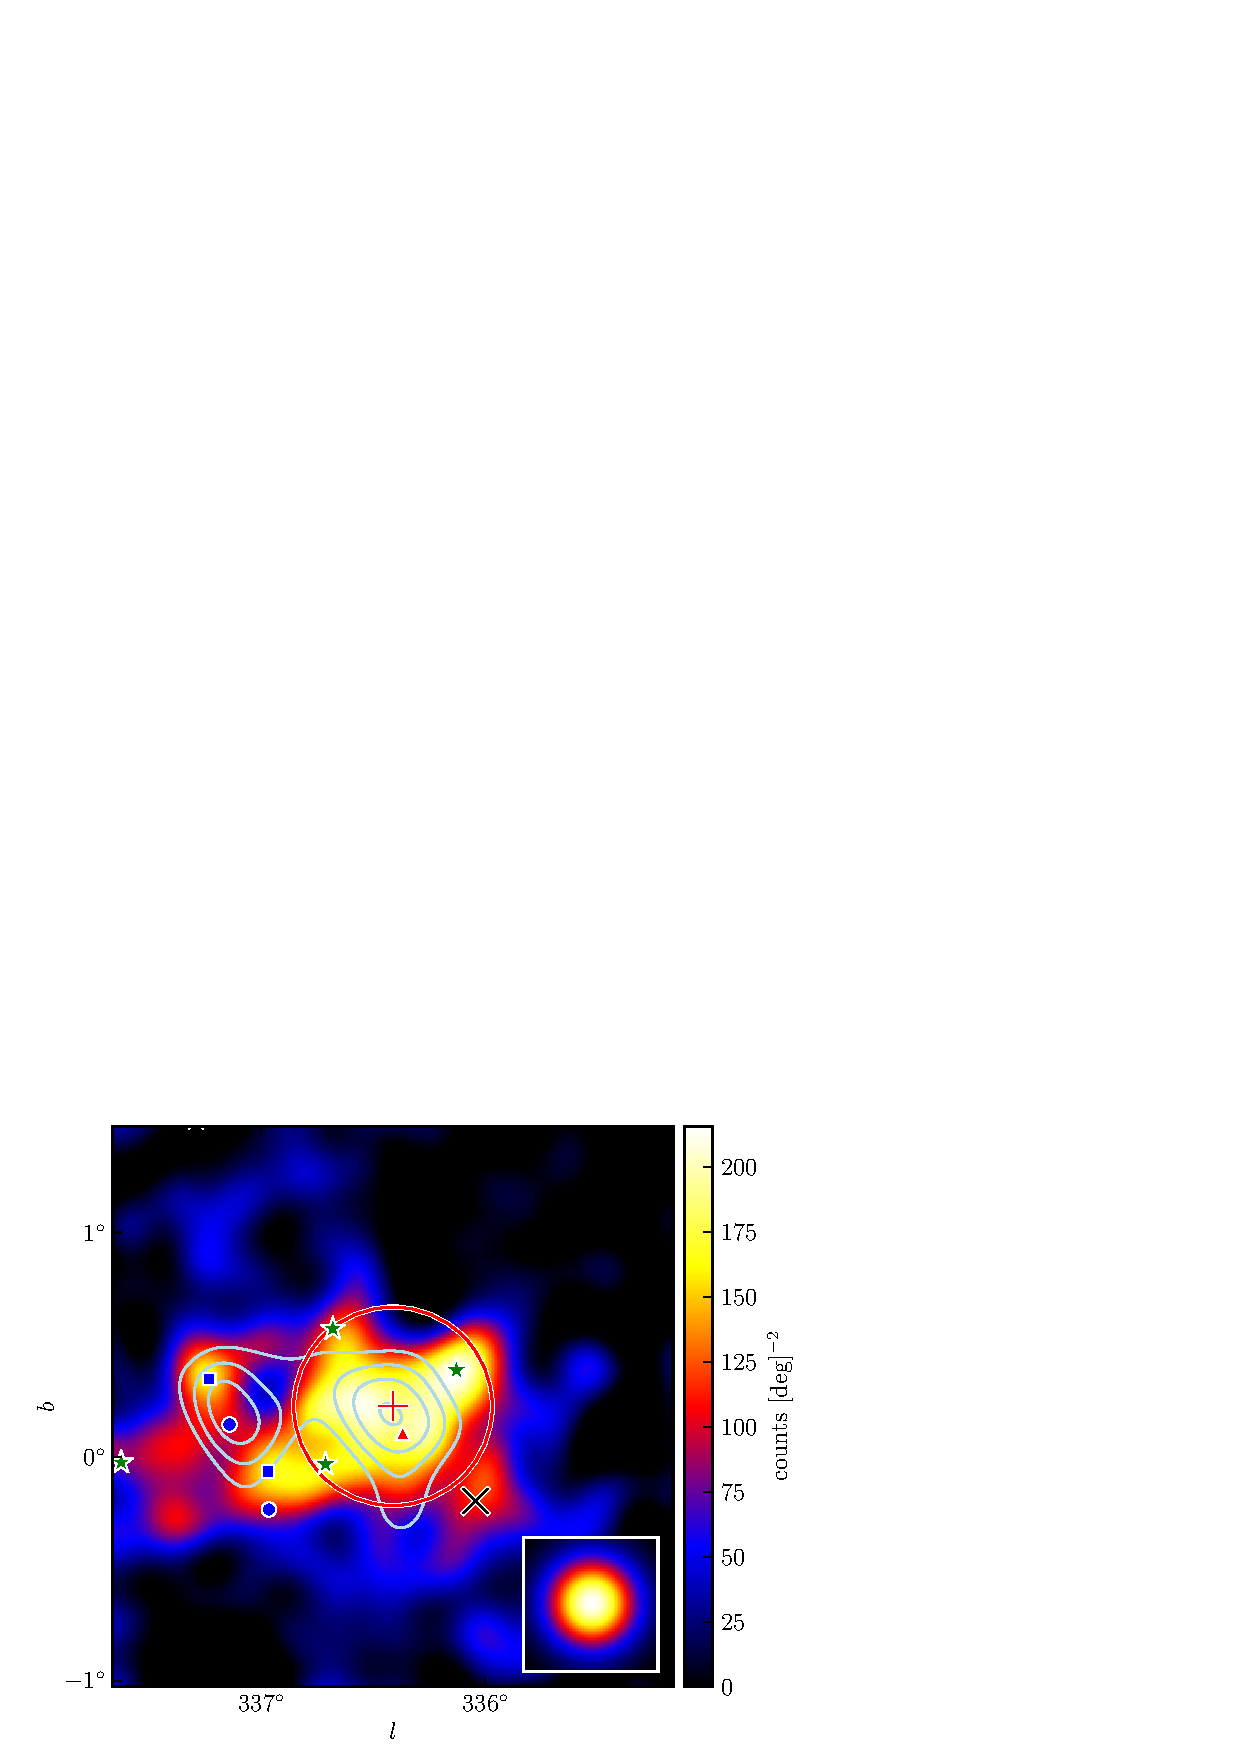
\includegraphics[scale=0.5]{plots/source_HESS_J1632-478_color.pdf}
    \column{.35\textwidth} 
    \begin{itemize}
      \item 10 GeV to 100 GeV
      \item  {\em XMM-Newton} point-like + extended emission
        ($32''\times15''$)
    \end{itemize}
  \end{columns}

  \begin{itemize}
      \item PWN? No pulsations (yet) in point-like X-ray source
        towards center of H.E.S.S source (Balbo+2010)
      \item Extended radio source in archival MGPS-2 data
    \end{itemize}

\end{frame}


\begin{frame}{Fig. 21: HESS\,J1837-069}
  \begin{columns}
    \column{.55\textwidth} 
    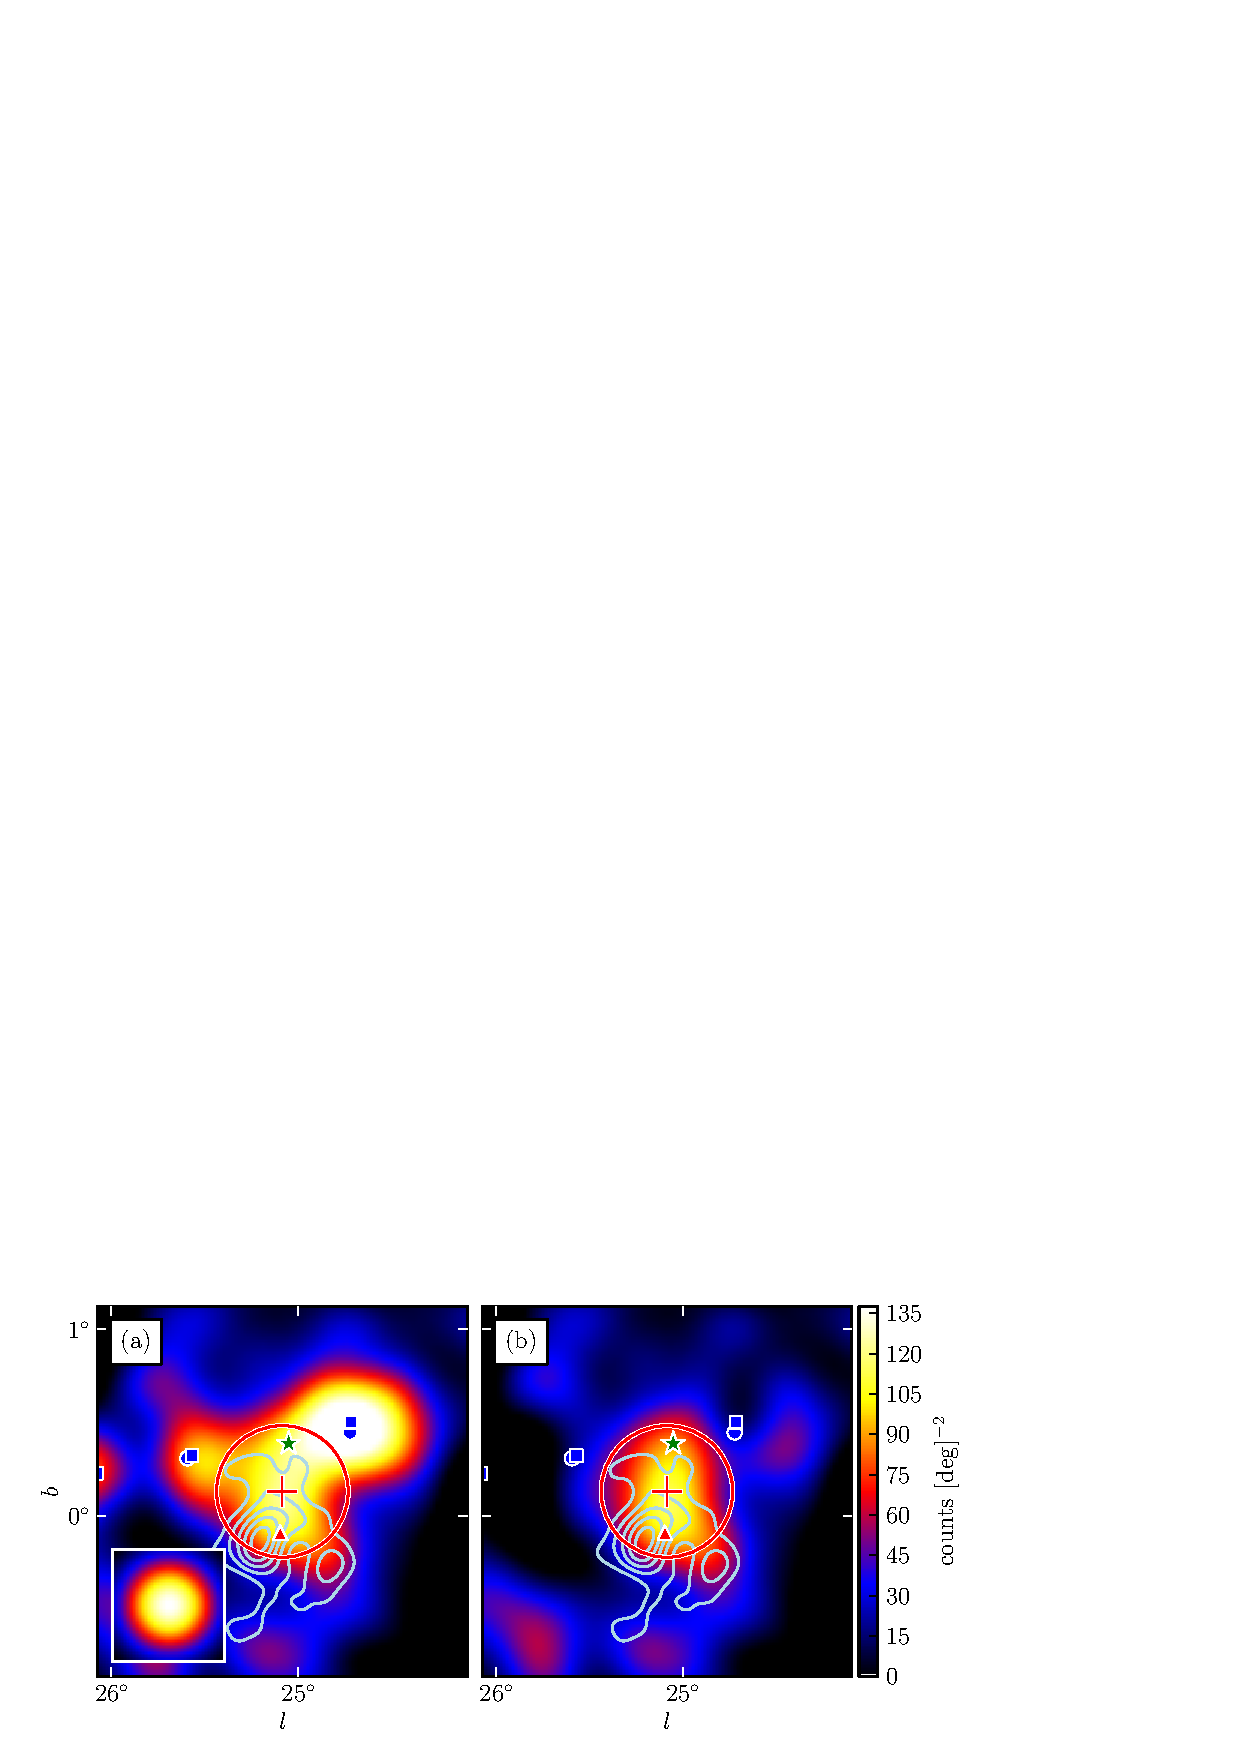
\includegraphics[scale=0.45]{plots/source_HESS_J1837-069_color.pdf}
    \column{.45\textwidth} 
    \begin{itemize}
      \item 10 GeV to 100 GeV
      \item Coincident with X-ray source
        AX\,J1838$-$0655 (Hertz \& Grindlay 1988)
      \item X-ray Pulsations: PSR\,J1838$-$0655 
    \end{itemize}
  \end{columns}
    \begin{itemize}
      \item also: X-ray PWN $\sim 2'$ 
        (Gotthelf \& Halpern 2008)
      \item $\gamma$-rays from PWN?
      \item Second X-ray source
        AX\,J1837.3$-$0652 resolved into
        point + extended component (no pulsations yet)
      \item $\gamma$-rays from multiple PWN
    \end{itemize}
\end{frame}


\begin{frame}{Fig. 18: SED of HESS Sources}
  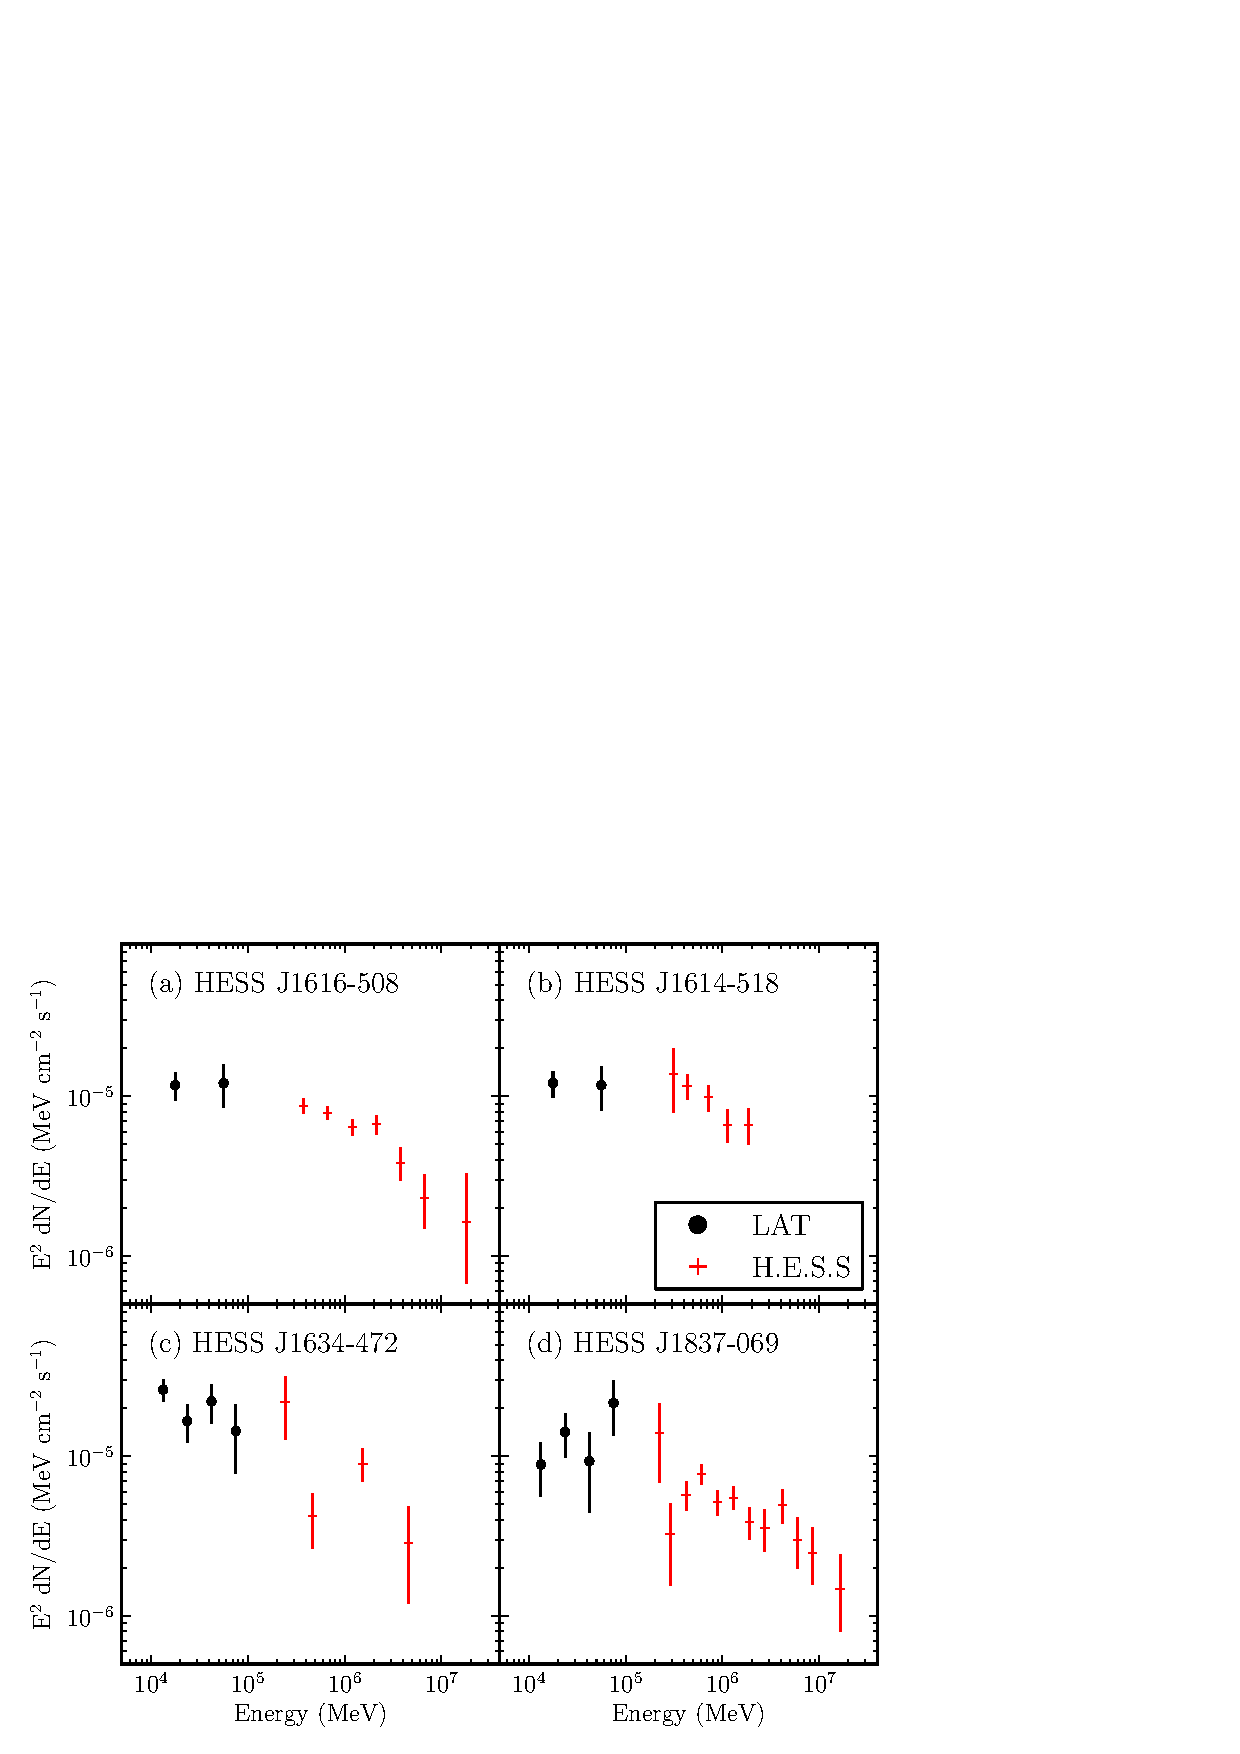
\includegraphics[scale=0.5]{plots/hess_seds_color.pdf}
\end{frame}

\begin{frame}{Fig. 20: RX J1713.7$-$3946}
  \includegraphics[scale=0.65]{plots/source_RX_J1713_7-3946_color.pdf}
  \begin{itemize}
  \item Beautiful GeV Image for E$>$10 GeV!
  \end{itemize}
\end{frame}


\begin{frame}{Table 4: New extended Sources}
    \includegraphics[scale=0.50]{plots/new_extended.pdf}
\end{frame}


\begin{frame}{Section 8: Extension Systematics}
  Test systematics due to not knowing PSF
  \begin{itemize}
    \item Compare best fit extension to 
      MC based PSF
    \item Use difference as systematic
    \item Small effect on extension, large effect on statistical 
      significance
    \item Probably too conservative\dots
  \end{itemize}
  Test systematics due to not knowing PSF
  \begin{itemize}
    \item Break up GALPROP diffuse model into multiple components 
    \item Fit each component locally
    \item Tests systematics due to imperfect diffuse modeling
  \end{itemize}
\end{frame}

\begin{frame}{Table 5: Dual Localization, alternate PSF, alternate Diffuse}
  \includegraphics[scale=0.45]{plots/alt_diff.pdf}
\end{frame}

\begin{frame}{Fig 23: Skymap of Extended Sources}
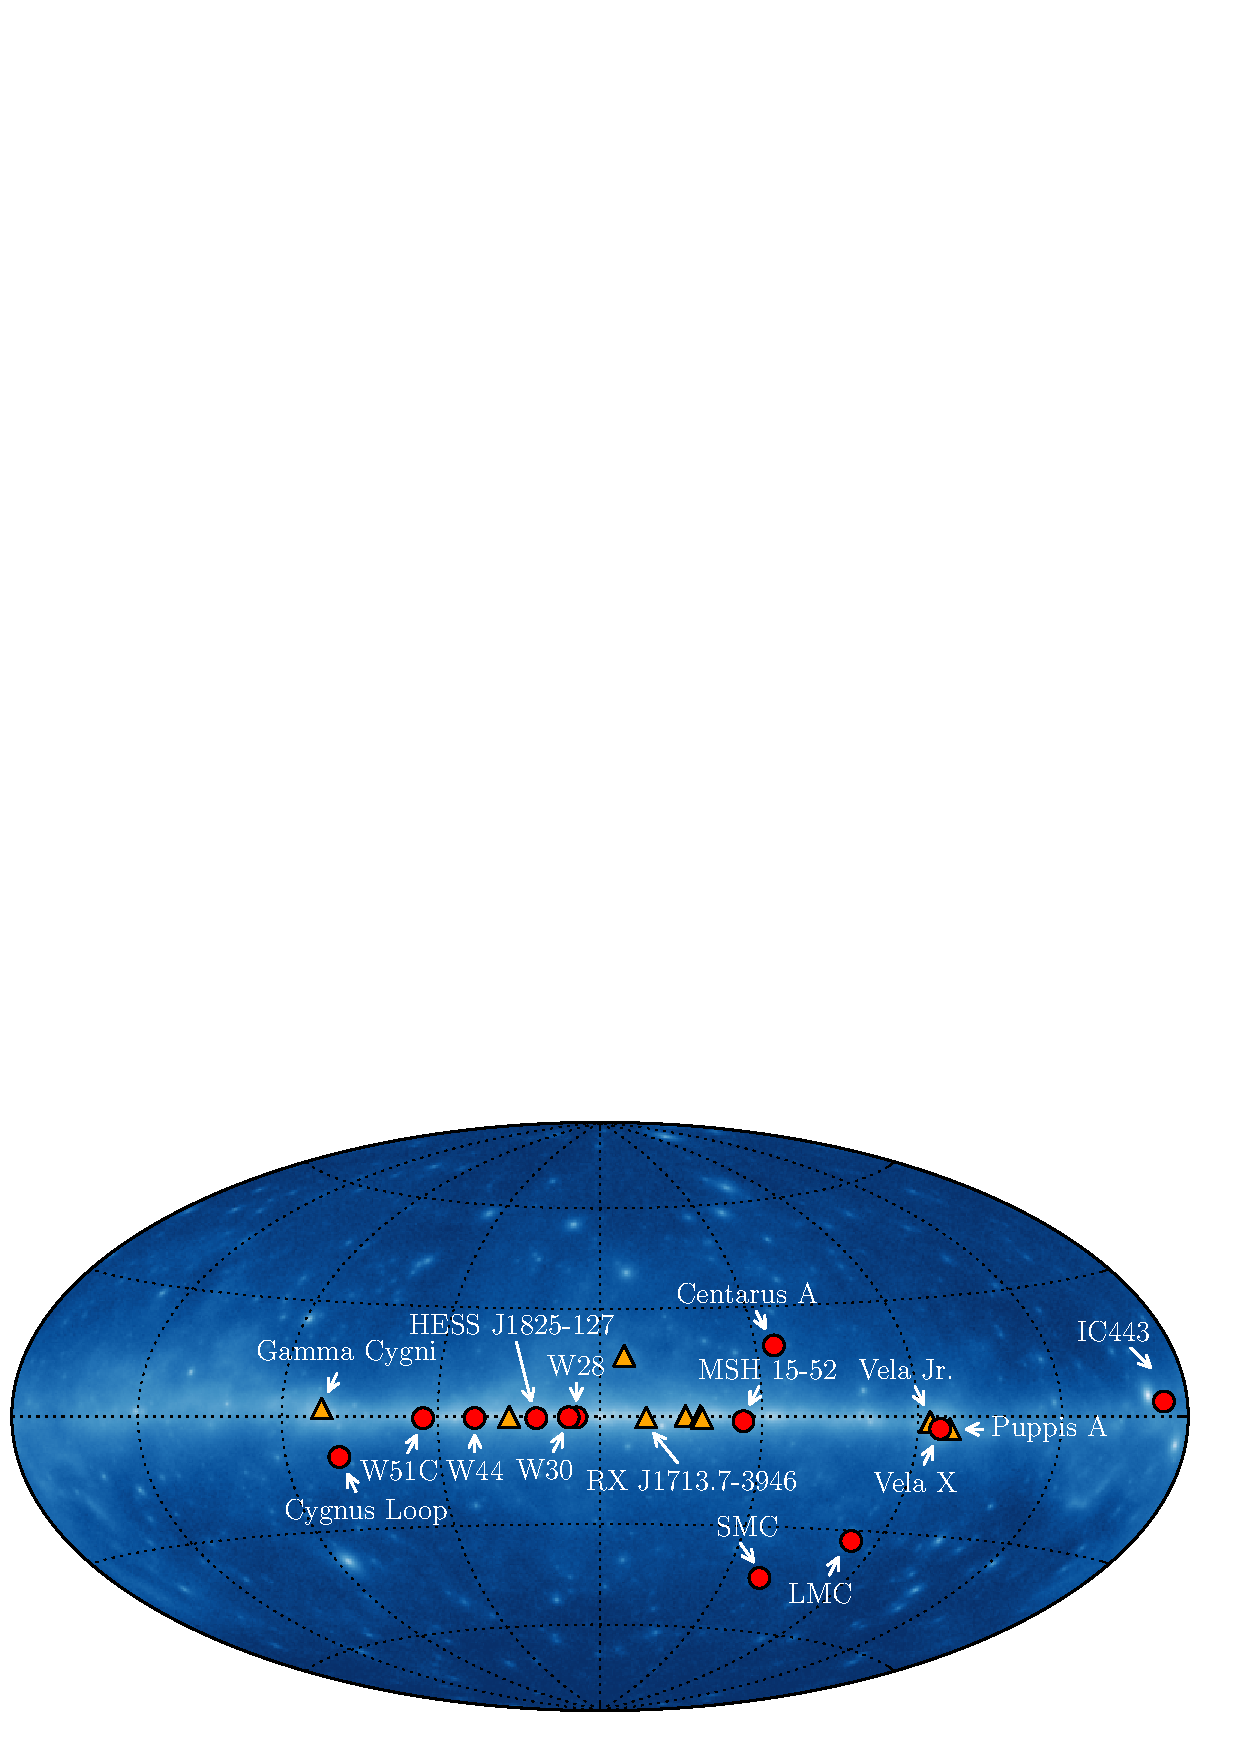
\includegraphics[scale=0.60]{plots/allsky_extended_sources_color.pdf}
\end{frame}

\begin{frame}{Fig 24: Compare GeV and TeV Sizes}
  \includegraphics[scale=0.60]{plots/gev_vs_tev_plot_color.pdf}
\end{frame}

\begin{frame}{Fig 25: GeV and TeV Sizes (cont)}
  \includegraphics[scale=0.60]{plots/gev_vs_tev_histogram_color.pdf}
\end{frame}

\begin{frame}{Fig 26: Distribution of Spectral Indices}
  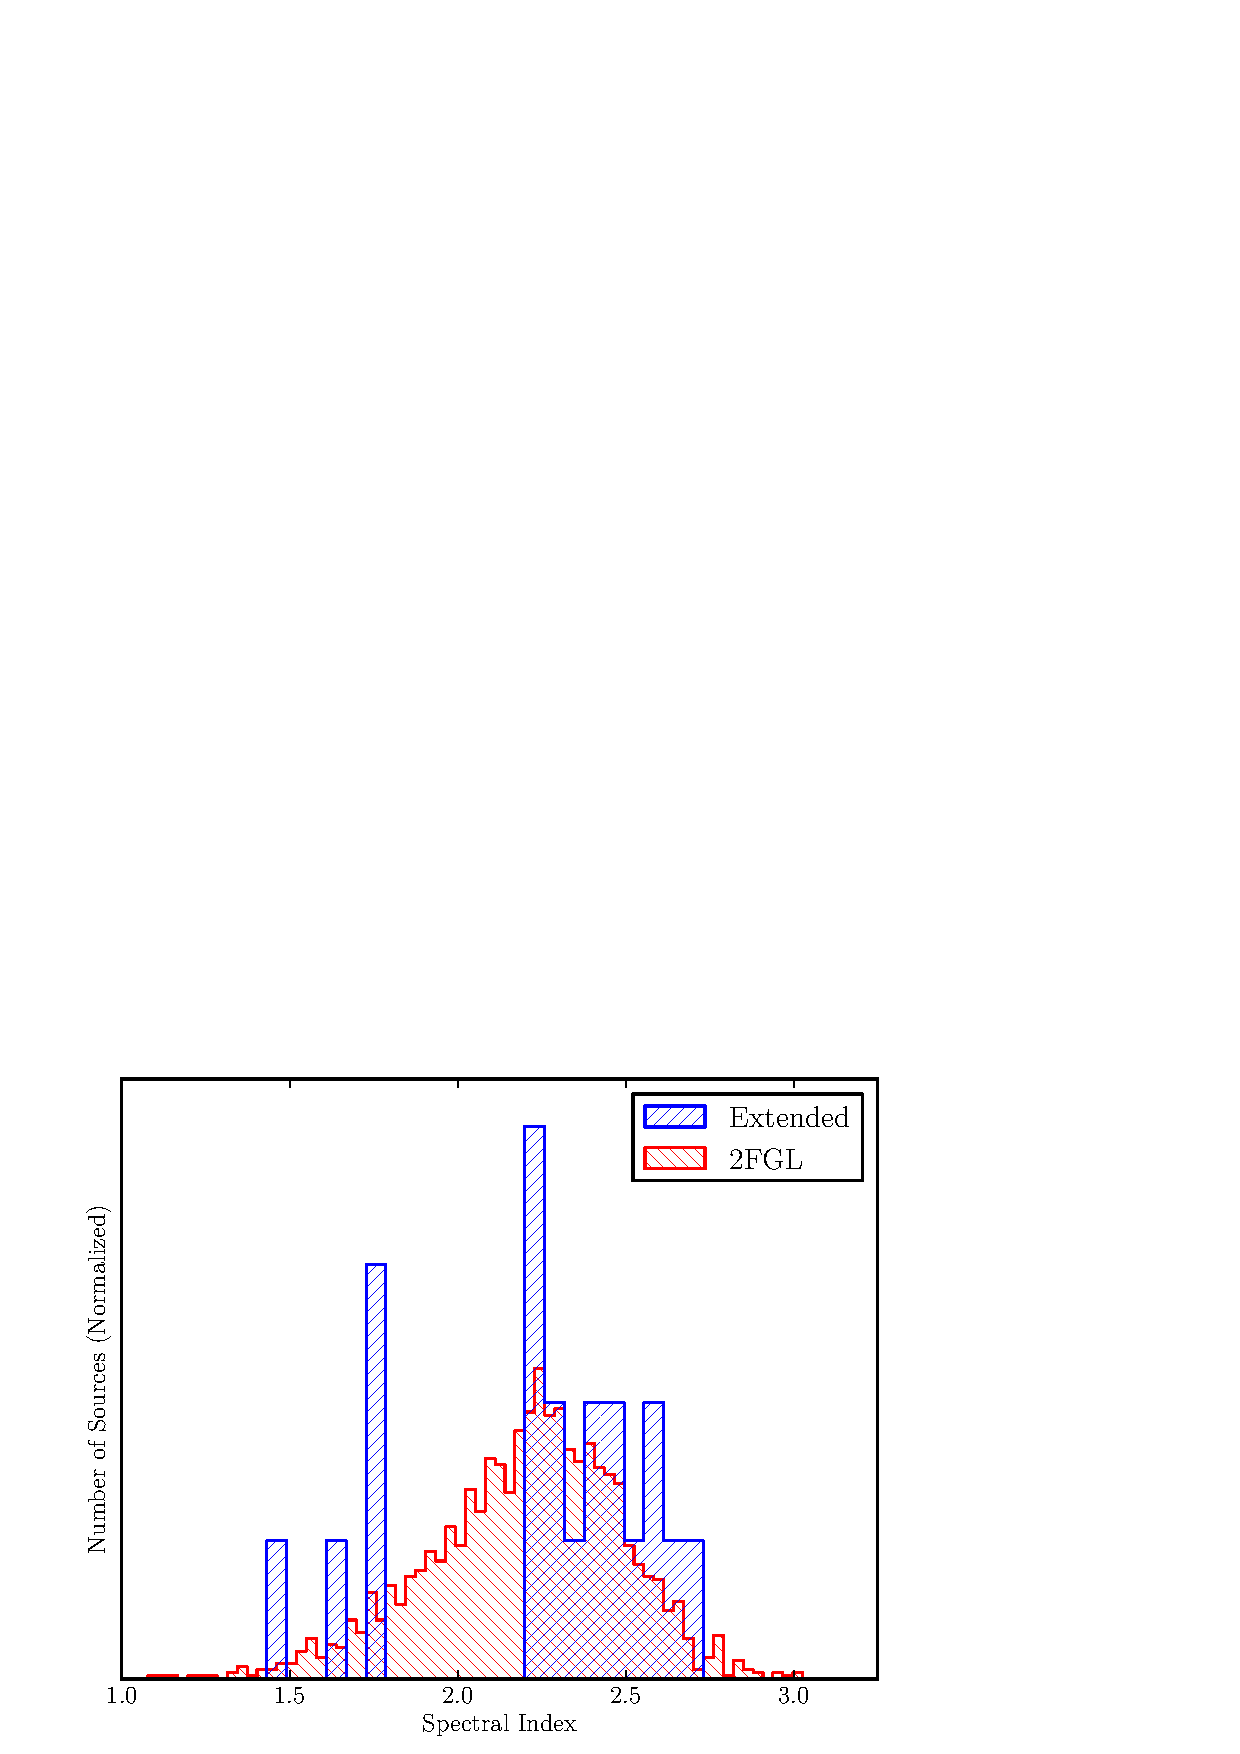
\includegraphics[scale=0.60]{plots/compare_index_2FGL_color.pdf}
\end{frame}

\begin{frame}{Thank you}
  See text for more details:
  \begin{itemize}
    \item
  \url{https://www-glast.stanford.edu/cgi-prot/pub_download?id=662}
  \end{itemize}
\end{frame}

\end{document}
